%==============================================================================
%  DRAFT -- IEEE Wireless Communications Letters style
%  Revised to align the formulation and MAML discussion with the reference
%  RIS-NOMA and RIS-ISAC papers while keeping the present simulation results.
%==============================================================================
\documentclass[10pt,journal]{IEEEtran}

\usepackage{graphicx}
\usepackage{epstopdf}
\usepackage{amsmath}
\usepackage{newtxtext,newtxmath}
\usepackage{bm}
\usepackage{booktabs}
\usepackage{url}
\usepackage[caption=false,font=footnotesize]{subfig}
\usepackage[ruled,vlined]{algorithm2e}
\usepackage{tikz}
\usepackage{pgfplots}
\pgfplotsset{compat=1.18}
\usetikzlibrary{arrows.meta,shapes.geometric,positioning}

\graphicspath{{figs/}}
\DeclareGraphicsExtensions{.pdf,.eps,.png,.jpg,.jpeg}

\newcommand{\Rdl}{R_{\mathrm{DL}}}
\newcommand{\Rsum}{R_{\mathrm{sum}}}
\newcommand{\bh}{\bm{h}}
\newcommand{\bw}{\bm{w}}
\newcommand{\bG}{\bm{G}}
\newcommand{\bH}{\bm{H}}
\newcommand{\bA}{\bm{A}}
\newcommand{\bPhi}{\bm{\Phi}}
\newcommand{\herm}{^{\mathsf{H}}}
\newcommand{\Cset}{\mathbb{C}}
\newcommand{\Eset}{\mathbb{E}}

\begin{document}

\title{Meta-Learning-Driven Joint Power Allocation and Phase-Shift Design
for RIS-Assisted NOMA-ISAC Systems}

% >>> PLACEHOLDER author block
\author{First~Author,~\IEEEmembership{Graduate~Student~Member,~IEEE,}
        Second~Author,~\IEEEmembership{Member,~IEEE,}
        and Third~Author,~\IEEEmembership{Senior~Member,~IEEE}
\thanks{Manuscript received \ldots; revised \ldots. This work was supported in
part by \ldots. \emph{(Corresponding author: First Author.)}}
\thanks{The authors are with the \ldots, \ldots\ (e-mail: author@univ.edu).}}

\markboth{IEEE Wireless Communications Letters,~Vol.~XX, No.~X, Month~2026}%
{Author \MakeLowercase{\textit{et al.}}: Meta-Learning-Driven Joint Power and Phase Design for RIS-Assisted NOMA-ISAC}

\maketitle

%==============================================================================
\begin{abstract}
This letter investigates a reconfigurable intelligent surface (RIS)-assisted
multiple-input single-output (MISO) integrated sensing and communication (ISAC)
system, where a base station (BS) simultaneously serves a near and a far user
via non-orthogonal multiple access (NOMA) while illuminating a sensing target.
We maximize a weighted communication-and-sensing throughput by jointly
optimizing the NOMA power-allocation coefficients and the RIS phase shifts,
subject to an aggregate communication QoS floor, individual near/far-user QoS
floors, and a sensing QoS constraint. To tackle the resulting non-convex problem,
a model-agnostic meta-learning (MAML)-based deep-learning algorithm is proposed.
A lightweight network predicts the low-dimensional power split, while an inner
optimizer adapts the high-dimensional RIS phase vector for each channel
realization. A first-order meta-update then trains the power map using the
phase-adapted channels, avoiding the unstable higher-order derivatives observed
in this high-SINR setting. Simulation results show
stable convergence, a strong RIS-aperture gain, and consistent improvements
against OMA, no-RIS, and partially optimized baselines.
\end{abstract}

\begin{IEEEkeywords}
Reconfigurable intelligent surface (RIS), integrated sensing and communication
(ISAC), non-orthogonal multiple access (NOMA), deep learning, meta-learning
(MAML), MISO.
\end{IEEEkeywords}

%==============================================================================
\section{Introduction}
\IEEEPARstart{I}{ntegrated} sensing and communication (ISAC) is a key enabler
for next-generation wireless systems because sensing and data transmission can
share spectrum, antennas, and radio-frequency hardware~\cite{liu2022isac}.
Power-domain non-orthogonal multiple access (NOMA) further allows multiple users
to occupy the same time-frequency resource by superposition coding and
successive interference cancellation (SIC), improving spectral efficiency when
users experience heterogeneous channel strengths~\cite{ding2017noma,sun2024noma}.
Reconfigurable intelligent surfaces (RISs) complement both ideas by controlling
the propagation environment through programmable passive elements, which is
particularly useful when the direct BS--user paths are blocked or severely
attenuated~\cite{basar2019ris,wu2020ris}.

Recent RIS-assisted ISAC studies have mainly relied on iterative optimization.
Hybrid active/passive beamforming was considered in~\cite{wang2025hybrid},
while~\cite{lyu2024crb} used block-coordinate optimization to improve sensing
accuracy and~\cite{ke2025rsma} investigated RIS-assisted rate-splitting ISAC.
For NOMA-assisted ISAC,~\cite{sun2024noma} established the benefits of sharing
resources between sensing and NOMA communication. Learning-based RIS design is
attractive because solving a non-convex phase-and-resource-allocation problem
from scratch for every channel realization can be costly. In this direction,
Zou \emph{et al.}~\cite{zou2023ml} applied machine learning and meta-learning to
RIS-assisted NOMA resource optimization, while the general meta-learning
literature shows how experience across related tasks can be used to obtain fast
adaptation on a new task~\cite{maml,hospedales2022meta}.

The remaining challenge in the considered RIS-NOMA-ISAC setting is that the
power split and RIS phases are tightly coupled: the three power coefficients are
low dimensional, whereas the RIS phase vector grows with $N$ and must react to
each channel realization. This motivates a bilevel design in which a compact
network learns the reusable power-allocation map and a short channel-specific
inner loop adapts the RIS phases.

The contributions of this letter are threefold. First, we formulate joint
power-allocation and RIS-phase optimization for MISO NOMA-ISAC with a
communication-cluster QoS constraint, individual near/far-user QoS constraints,
and a sensing QoS constraint. The individual constraints prevent a strong user
from masking a weak user behind an acceptable NOMA sum rate. Second, we develop
a first-order MAML-based bilevel solver in which the power-allocation network is
trained across channel realizations after RIS-phase adaptation; the formulation
therefore combines reusable learning with a small fixed online optimization
budget. Third, we characterize the convergence limitation and online complexity,
and evaluate the design against RIS/no-RIS, NOMA/OMA, and partial-optimization
baselines using the same channel model and held-out test procedure.

%==============================================================================
\section{System Model and Problem Formulation}\section{System Model and Problem Formulation}

\begin{figure}[t]
\centering
\IfFileExists{figs/fig_system_model.eps}{%
  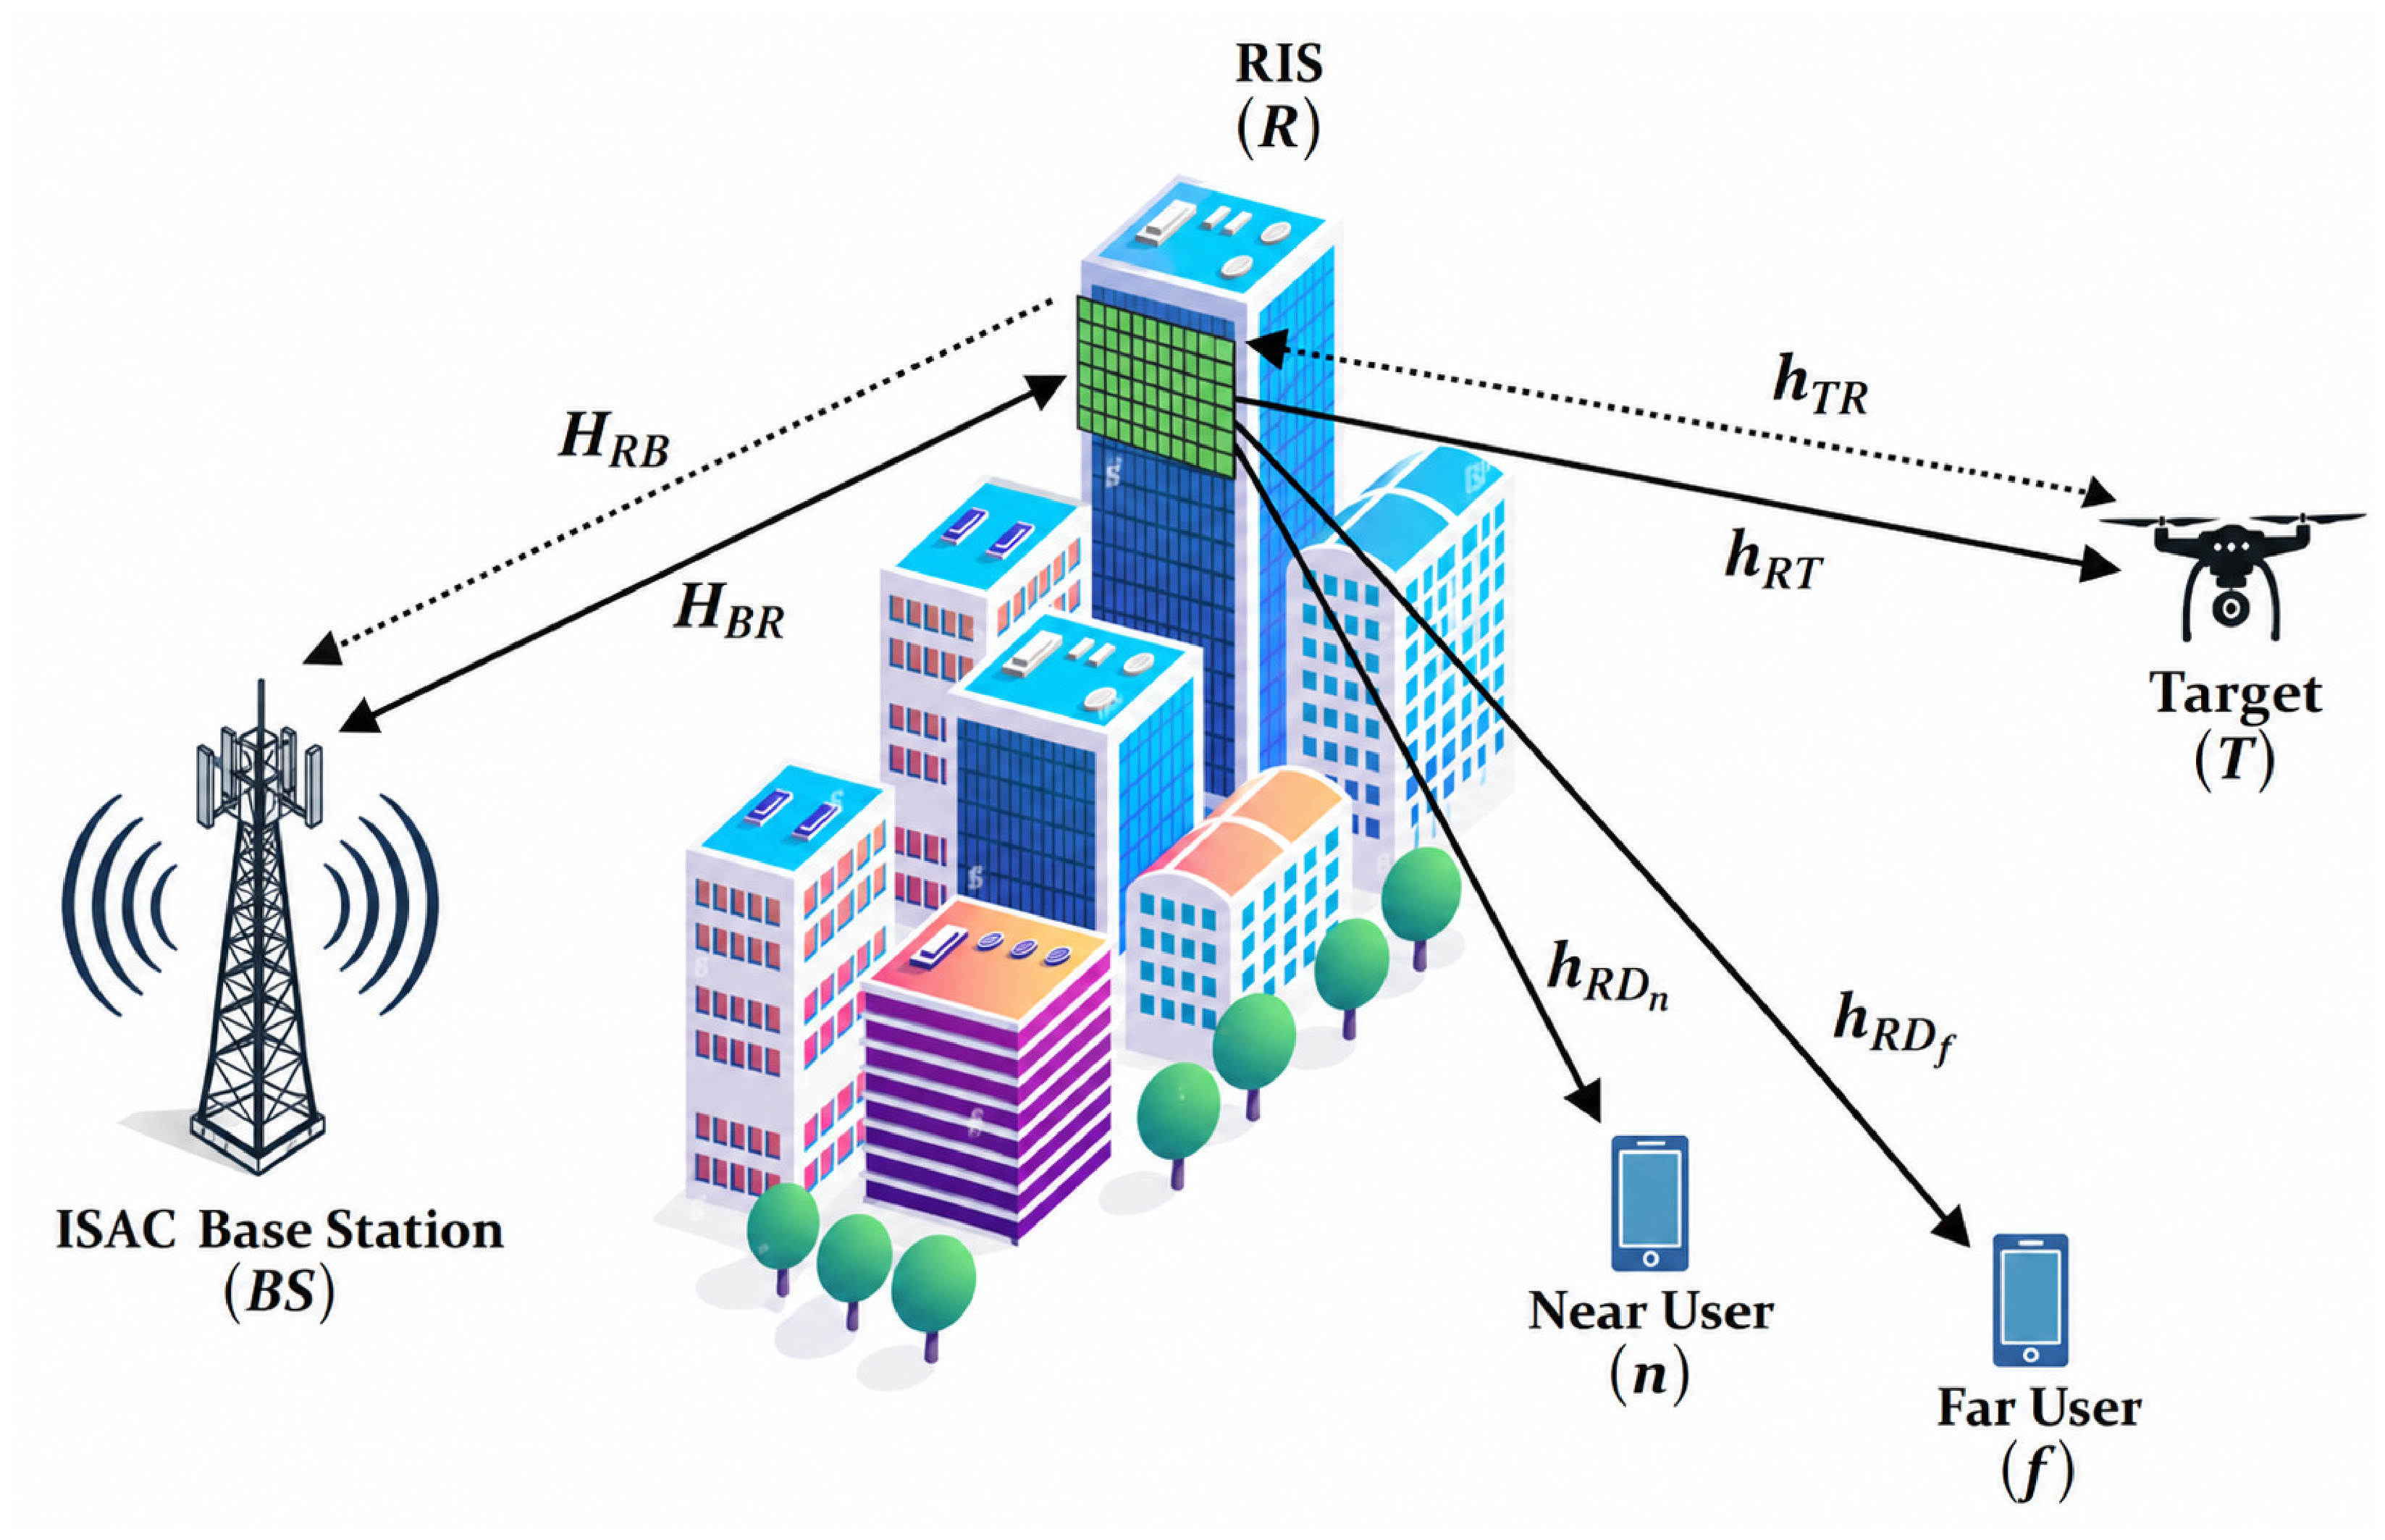
\includegraphics[width=\columnwidth]{fig_system_model}%
}{%
  \IfFileExists{figs/fig_system_model.jpg}{%
    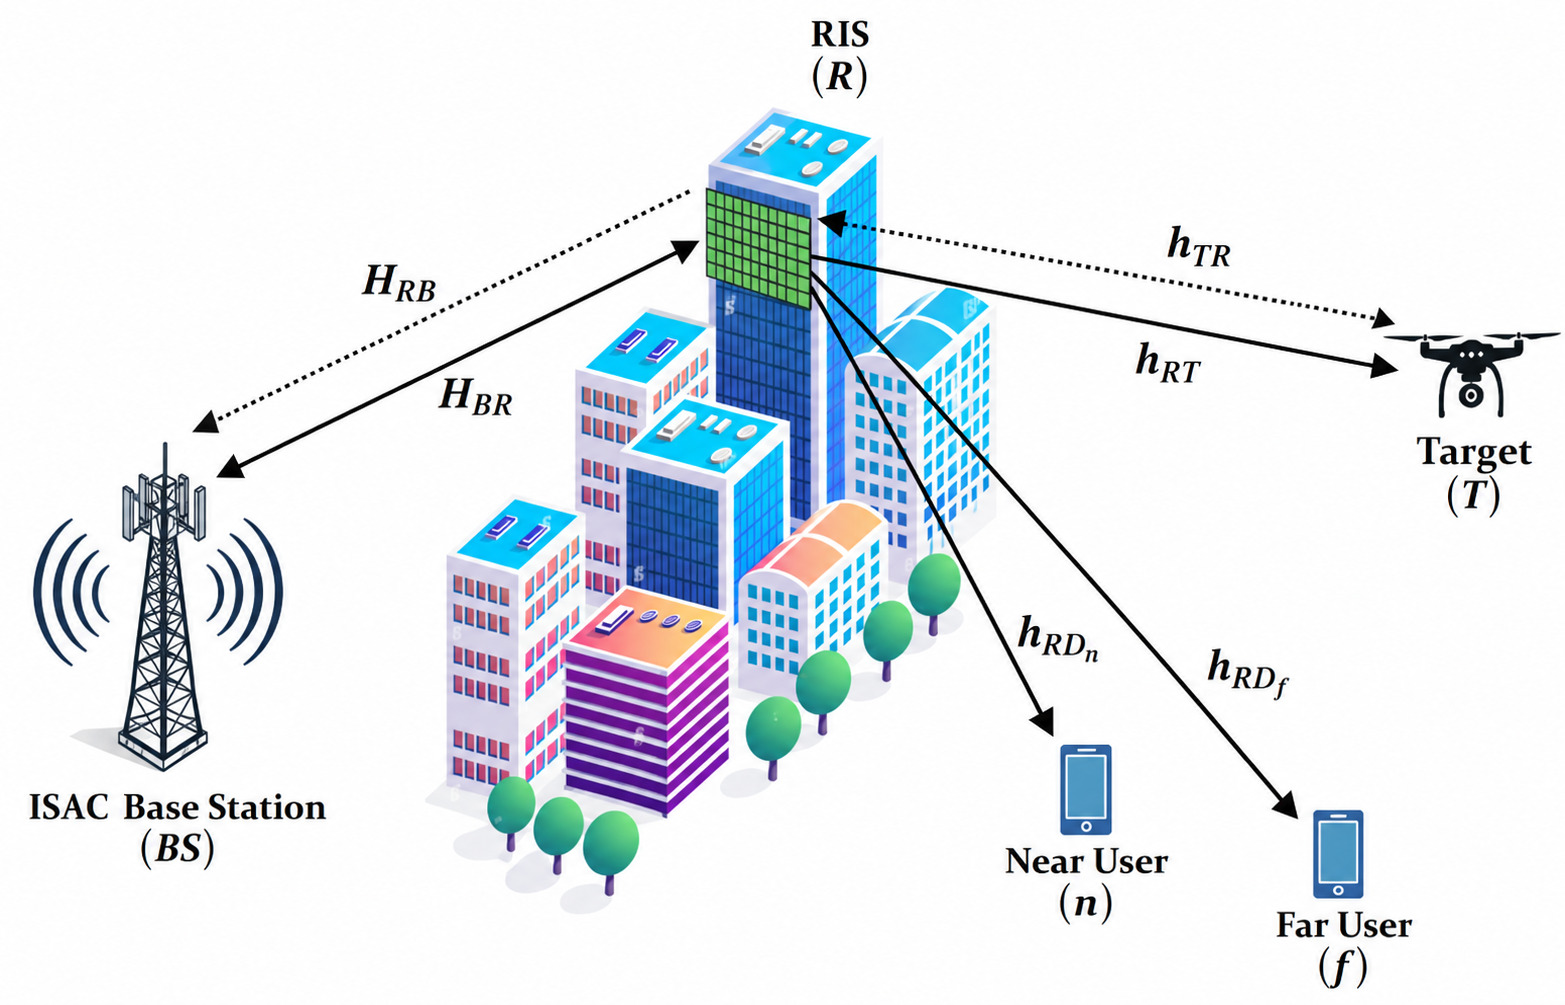
\includegraphics[width=\columnwidth]{fig_system_model.jpg}%
  }{%
    \fbox{\parbox[c][28mm][c]{0.96\columnwidth}{\centering
    System-model artwork placeholder. Upload \texttt{figs/fig\_system\_model.jpg}
    or the EPS version supplied with the revision.}}%
  }%
}
\caption{RIS-assisted MISO NOMA-ISAC system. The BS--RIS forward and reciprocal
channels are denoted by $\bH_{BR}$ and $\bH_{RB}$, the RIS--user channels by
$\bh_{RD_n}$ and $\bh_{RD_f}$, and the sensing links by $\bh_{RT}$ and
$\bh_{TR}$.}
\label{fig:system}
\end{figure}

\subsection{System Model}
As illustrated in Fig.~\ref{fig:system}, an $M$-antenna ISAC BS serves a
single-antenna near user $n$ and far user $f$ while illuminating a point target
through an $N$-element RIS. The coefficient of RIS element $i$ is written as
\begin{equation}
v_i=\rho_i e^{j\phi_i},\qquad 0\leq\rho_i\leq1,\quad \phi_i\in[0,2\pi),
\end{equation}
and $\bPhi=\operatorname{diag}(v_1,\ldots,v_N)$. The formulation keeps
$\rho_i$ symbolic; the ideal passive-RIS value used in the simulations is
reported only in Table~\ref{tab:system}.

\subsubsection{Channel Model}
Let $\bH_{BR}\in\Cset^{N\times M}$ denote the BS--RIS channel and let
$\bH_{RB}$ denote the reciprocal RIS--BS channel. For user
$k\in\{n,f\}$, $\bh_{RD_k}\in\Cset^N$ denotes the RIS--user channel. The
effective user channel is
\begin{equation}
\bh_k=\bH_{RB}\bPhi\bh_{RD_k}\in\Cset^M. \label{eq:cascade}
\end{equation}
The direct BS--user paths are blocked in the RIS-assisted data set, so the
cascaded term dominates. For the sensing path, $\bh_{RT}$ and $\bh_{TR}$
denote the RIS--target and target--RIS links, respectively. A rank-one
round-trip target response is modeled as
\begin{equation}
\bG_T=\sqrt{\beta_T}
(\bH_{RB}\bPhi\bh_{TR})
(\bh_{RT}\herm\bPhi\bH_{BR}), \label{eq:sensingchannel}
\end{equation}
where $\beta_T$ is the target/path-gain coefficient. Numerical values for
$\beta_T$, path loss, and fading are deliberately kept out of the model
equations and are listed in Section~IV.

\subsubsection{NOMA Communication and Sensing Model}
The transmitted signal is
\begin{equation}
\bm{x}=\left(\sqrt{a_nP}s_n+\sqrt{a_fP}s_f\right)\bw_c
       +\sqrt{a_TP}\bw_Ts_T, \label{eq:tx}
\end{equation}
where $\bm a=[a_n,a_f,a_T]$ is the near-user, far-user, and sensing power
split, $a_n+a_f+a_T=1$, and all entries are nonnegative. The unit-norm common
communication beam is parameterized without hard-coded numerical weights as
\begin{equation}
\bw_c=
\frac{\mu_f\bh_f+\mu_n\bh_n}
{\|\mu_f\bh_f+\mu_n\bh_n\|},\qquad
\mu_f,\mu_n\ge0,\quad \mu_f+\mu_n=1, \label{eq:wc}
\end{equation}
where $\mu_f$ and $\mu_n$ control the far/near steering emphasis. Both NOMA
users share $\bw_c$ and are separated through SIC~\cite{ding2017noma,zou2023ml}.

For sensing, define $\bH_u=[\bh_n,\bh_f]$ and the leakage-aware matrix
\begin{equation}
\bA_T=\bG_T\herm\bG_T-\lambda_L\bH_u\bH_u\herm. \label{eq:wTmat}
\end{equation}
The sensing beam is the normalized dominant eigenvector,
$\bw_T=\bm v_{\max}(\bA_T)/\|\bm v_{\max}(\bA_T)\|$. Thus
$\lambda_L$ is a tunable leakage-control parameter rather than a numerical
constant embedded in the system model~\cite{wang2025hybrid,lyu2024crb}.

With $g_{kj}=|\bh_k\herm\bw_j|^2$, the SINRs used by the implementation are
\begin{align}
\gamma_f &= \frac{a_fg_{ff}P}{a_ng_{ff}P+a_Tg_{fT}P+\sigma^2}, \label{eq:gf}\\
\gamma_n &= \frac{a_ng_{nn}P}{a_Tg_{nT}P+\sigma^2}, \label{eq:gn}\\
\gamma_s &= \frac{a_T|\bm u_T\herm\bG_T\bw_T|^2P}{\sigma^2}, \label{eq:gs}
\end{align}
where $\sigma^2$ is the receiver-noise power and $\bm u_T$ is the sensing
receive combiner. The rates are $R_k=\log_2(1+\gamma_k)$,
$k\in\{n,f,s\}$. The weighted ISAC objective is
\begin{equation}
\Rdl=\omega_c(R_n+R_f)+\omega_sR_s,\qquad \omega_c+\omega_s=1.
\label{eq:rdl}
\end{equation}
The sum $R_n+R_f$ is the NOMA-cluster spectral efficiency, while
$\omega_c$ and $\omega_s$ express the communication/sensing design priority.
Their numerical settings are reported with the simulation parameters.

\subsection{Problem Formulation}\label{sec:prob}
We jointly optimize the power split $\bm{a}$ and RIS phases
$\bm{\phi}=[\phi_1,\ldots,\phi_N]$. The communication sum rate is retained as a
cluster-level QoS measure, while individual user constraints are added in the
same spirit as the per-device QoS constraint in (9b) of~\cite{zou2023ml}. The
resulting problem is
\begin{subequations}\label{eq:prob}
\begin{align}
\text{(P1)}\quad \max_{\bm{a},\bm{\phi}}\quad & \Rdl \label{eq:obj}\\
\text{s.t.}\quad
& R_n+R_f\geq R_{\mathrm{th},c}, \label{eq:qosc}\\
& R_k\geq R_{\mathrm{th},k},\quad k\in\{n,f\}, \label{eq:qosu}\\
& R_s\geq R_{\mathrm{th},s}, \label{eq:qoss}\\
& a_n+a_f+a_T=1,\quad a_n,a_f,a_T\geq0, \label{eq:simplex}\\
& |e^{j\phi_i}|=1,\quad i=1,\ldots,N. \label{eq:unit}
\end{align}
\end{subequations}
The aggregate constraint~\eqref{eq:qosc} is useful because the two NOMA users
share one time-frequency resource block, so $R_n+R_f$ directly measures the
communication service delivered by the cluster. It also matches the
cluster-level QoS term used by the implemented training loss. On its own,
however, a sum threshold is insufficient: a very large near-user rate could
compensate for an unacceptable far-user rate. Constraint~\eqref{eq:qosu}
therefore adds the individual protection requested in the formulation, exactly
analogous to writing a QoS condition for each device as in (9b) of
\cite{zou2023ml}. Thus, the sum threshold controls aggregate communication
quality while the individual thresholds prevent user starvation. The sensing
requirement is enforced separately by~\eqref{eq:qoss}. The ideal-RIS assumption
$\beta_i=1$ is fixed rather than optimized, and the phase parameterization
$e^{j\phi_i}$ enforces unit modulus automatically.

Problem~(P1) remains non-convex because the power variables and RIS phases are
coupled through the cascaded channels. We therefore enforce the QoS conditions
through penalty terms during learning, while the softmax output enforces the
power simplex exactly.

%==============================================================================
\section{Proposed MAML-Based Solution}
\subsection{Motivation for Meta-Learning}
The optimization variables react on two different time and dimensional scales.
The power vector has only three entries and exhibits reusable structure across
related channel realizations, whereas the $N$ RIS phases are strongly
channel-specific. A conventional alternating optimizer would solve the coupled
non-convex problem again for every realization, while a purely one-shot neural
network must learn a direct map to a high-dimensional phase vector and can be
sensitive to distribution shifts.

Meta-learning is well suited to this structure because it learns across a
family of related tasks and is explicitly designed for fast adaptation on a
new task~\cite{maml,hospedales2022meta}. Here each channel realization is
treated as an adaptation task: the outer learner captures the reusable
power-allocation rule, and the inner loop spends a small fixed number of
gradient steps adapting the RIS phase to the current channel. This
learning-plus-adaptation structure follows the motivation of RIS-NOMA
meta-learning in~\cite{zou2023ml}, but is specialized to the joint
communication-and-sensing objective and its QoS penalties. The implemented
first-order update further avoids storing the full higher-order derivative
graph, reducing training memory and improving numerical robustness
\cite{fallah2020maml,ji2022maml}.

\subsection{Feature Map and Power-Allocation Network}\label{sec:feat}
For a given phase vector, the cascaded channels and the six effective gains
$\{g_{nn},g_{ff},g_{sT},g_{fn},g_{fT},g_{nT}\}$ are computed. They are converted
to dB and concatenated with the communication/sensing QoS levels and the SNR
budget, giving a nine-dimensional input feature vector $\bm z$. The power
network contains three hidden layers with 256 neurons per layer, LayerNorm and
LeakyReLU activations, followed by a three-neuron softmax head. Hence
\begin{equation}
\bm a=\operatorname{softmax}(f_{\bm\theta}(\bm z)),
\end{equation}
which enforces $a_n+a_f+a_T=1$ and $a_k\geq0$ by construction.

\subsection{Joint Power-Allocation and Phase Adaptation}
For a channel sample and the current phase vector $\bm\phi^{(j)}$, the network
first predicts
\begin{equation}
\bm a^{(j)}=\operatorname{softmax}
\left(f_{\bm\theta}(\bm z(\bm\phi^{(j)}))\right). \label{eq:powerpred}
\end{equation}
The implemented constrained loss is
\begin{align}
\ell^{(j)}={}&-\Rdl
+\lambda_c\big(R_{\mathrm{th},c}-R_n-R_f\big)_+
+\lambda_s\big(R_{\mathrm{th},s}-R_s\big)_+ \notag\\
&+\lambda_n\big(R_{\mathrm{th},n}-R_n\big)_+
+\lambda_f\big(R_{\mathrm{th},f}-R_f\big)_+, \label{eq:sampleloss}
\end{align}
where $(x)_+=\max(x,0)$. Equation~\eqref{eq:sampleloss} makes explicit why the
aggregate and individual communication thresholds coexist: $\lambda_c$ protects
cluster throughput, whereas $\lambda_n$ and $\lambda_f$ penalize starvation of
either user.

The two update equations below describe the inner phase adaptation and the
outer meta-update. The index $j\in\{0,\ldots,K-1\}$ denotes the inner step,
$K$ is the fixed number of RIS-adaptation steps, $\eta_{\phi}$ is the inner
phase-learning rate, $\bm\theta$ denotes the parameters of the power-allocation
network, $\alpha$ is the outer learning rate, and $B$ is the mini-batch size.
The penalty coefficients $\lambda_c,\lambda_s,\lambda_n,\lambda_f$ control the
strength of the aggregate-communication, sensing, near-user, and far-user QoS
penalties, respectively.

The RIS phase is represented by
$\theta_i=e^{j\phi_i}=\cos\phi_i+j\sin\phi_i$, so unit modulus is satisfied for
any real $\phi_i$. For each channel, the phase vector is randomly initialized
and adapted for $K$ steps using Adam on~\eqref{eq:sampleloss},
\begin{equation}
\bm\phi^{(j+1)}=\operatorname{Adam}_{\phi}
\left(\bm\phi^{(j)},\nabla_{\bm\phi^{(j)}}\ell^{(j)};\eta_{\phi}\right),
\label{eq:inner}
\end{equation}
with inner learning rate $\eta_{\phi}$. Since the effective gains change after
every phase update, the feature vector and power split are recomputed at each
inner step.

\subsection{First-Order Meta-Update}
After the $K$ phase-adaptation steps, the final rates and loss are recomputed at
$\bm\phi^{(K)}$. The implementation uses a first-order MAML approximation: the
adapted phase is treated as fixed during the outer network update rather than
backpropagating second-order derivatives through the entire Adam trajectory.
The outer update is therefore
\begin{equation}
\bm\theta\leftarrow\bm\theta-\alpha
\nabla_{\bm\theta}\frac{1}{B}\sum_{b=1}^{B}
\ell_b\big(\bm\theta,\bm\phi_b^{(K)}\big), \label{eq:outer}
\end{equation}
where the gradient is evaluated at the phase-adapted state
$\bm\phi_b^{(K)}$. Thus, Eq.~\eqref{eq:inner} changes the channel-specific
RIS variable while Eq.~\eqref{eq:outer} updates the reusable network
parameters. The former uses $\eta_{\phi}$ and $K$; the latter uses the
mini-batch size $B$ and outer rate $\alpha$. This retains the key meta-learning idea--the
power map is trained on channels after per-instance RIS adaptation--while
avoiding the memory and numerical burden of the full higher-order graph. In the
implemented fair, high-SINR configuration, the full second-order path was found
to produce unstable/non-finite meta-gradients, which motivated the first-order
variant.

\begin{figure*}[t]
\centering
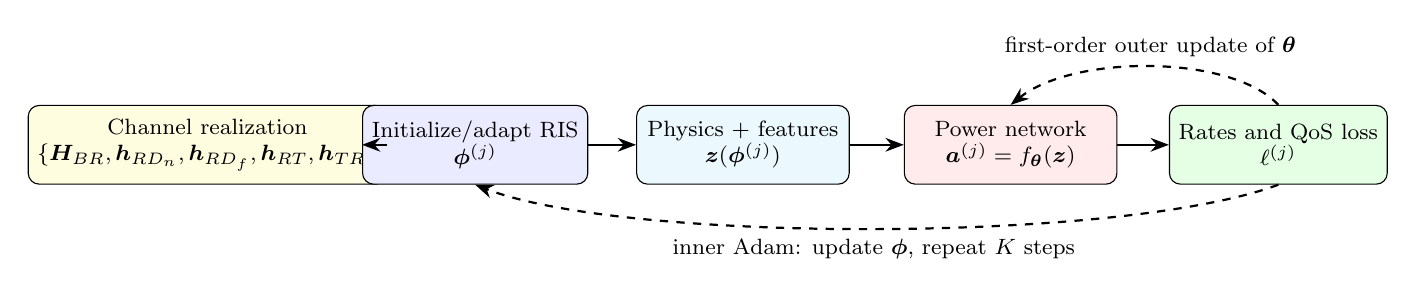
\begin{tikzpicture}[
  >=Stealth,
  box/.style={draw,rounded corners,align=center,minimum width=27mm,
              minimum height=10mm,font=\footnotesize},
  arr/.style={->,thick},
  loop/.style={->,thick,dashed}
]
\node[box,fill=yellow!12] (ch) at (0,0) {Channel realization\\
$\{\bH_{BR},\bh_{RD_n},\bh_{RD_f},\bh_{RT},\bh_{TR}\}$};
\node[box,fill=blue!8] (ph) at (3.4,0) {Initialize/adapt RIS\\$\bm\phi^{(j)}$};
\node[box,fill=cyan!8] (ft) at (6.8,0) {Physics + features\\$\bm z(\bm\phi^{(j)})$};
\node[box,fill=red!8] (nn) at (10.2,0) {Power network\\$\bm a^{(j)}=f_{\bm\theta}(\bm z)$};
\node[box,fill=green!10] (ls) at (13.6,0) {Rates and QoS loss\\$\ell^{(j)}$};
\draw[arr] (ch) -- (ph);
\draw[arr] (ph) -- (ft);
\draw[arr] (ft) -- (nn);
\draw[arr] (nn) -- (ls);
\draw[loop] (ls.south) .. controls (11.6,-1.25) and (5.3,-1.25) ..
 node[below,font=\footnotesize] {inner Adam: update $\bm\phi$, repeat $K$ steps} (ph.south);
\draw[loop] (ls.north) .. controls (13.0,1.15) and (11.0,1.15) ..
 node[above,font=\footnotesize] {first-order outer update of $\bm\theta$} (nn.north);
\end{tikzpicture}
\caption{First-order MAML-based joint power/phase design. The inner loop adapts
the channel-specific RIS phase and recomputes the power split; after $K$ inner
steps, the outer update trains the reusable power-allocation network. The
two-column layout separates the inner and outer update paths to avoid overlap.}
\label{fig:maml}
\end{figure*}

\subsection{Training and Prediction Procedure}
Algorithm~\ref{alg:maml} summarizes the implementation. At inference, the same
$K$-step phase adaptation is performed for an unseen channel and the final
softmax output provides the power allocation. Thus prediction is not a pure
one-shot neural-network call; it is a short learned-plus-optimization procedure
that trades a small fixed online cost for substantially better phase adaptation.

\begin{algorithm}[t]
\SetAlgoLined
\DontPrintSemicolon
\KwIn{channel data; inner steps $K$; inner Adam rate $\eta_{\phi}$; outer rate
$\alpha$; penalties $\lambda_c,\lambda_s,\lambda_n,\lambda_f$.}
\KwOut{trained power-map parameters $\bm\theta^\star$.}
Initialize $\bm\theta$\;
\While{not converged}{
 Sample a mini-batch of $B$ channels\;
 \ForEach{channel $b$}{
   Initialize $\bm\phi_b^{(0)}\sim\mathcal U([0,2\pi)^N)$\;
   \For{$j=0$ \KwTo $K-1$}{
     Compute phase-dependent channels/gains and $\bm z_b^{(j)}$\;
     Predict $\bm a_b^{(j)}$ using~\eqref{eq:powerpred}\;
     Evaluate $R_n,R_f,R_s$ and~\eqref{eq:sampleloss}\;
     Update $\bm\phi_b^{(j+1)}$ with inner Adam\;
   }
   Recompute $\bm a_b^{(K)}$ and final loss at the adapted phase\;
 }
 Update $\bm\theta$ with Adam using the first-order gradient in~\eqref{eq:outer}\;
}
Select $\bm\theta^\star$ by validation score\;
\caption{First-order MAML-based power and RIS-phase optimization}
\label{alg:maml}
\end{algorithm}

\subsection{Convergence Analysis}
A global convergence guarantee is not claimed. The objective is non-convex, the
unit-modulus RIS parameterization couples all rates through the cascaded channel,
and the hinge penalties in~\eqref{eq:sampleloss} are non-smooth exactly at the
QoS boundaries. Moreover, as discussed for the related RIS-NOMA MAML method in
\cite{zou2023ml}, standard smooth MAML convergence theorems do not directly
cover an architecture in which the inner and outer loops optimize different
variables. Our first-order approximation further discards the higher-order
dependence of the adapted phase on $\bm\theta$. Consequently, convergence is
assessed empirically: the inner Adam loop is run for a fixed number of steps and
the outer training curve is checked for a stable loss/rate plateau across the
reported hyperparameter settings.

\subsection{Computational Complexity}
Let $P_{\bm\theta}$ denote the power-network parameter count. With nine inputs,
three 256-unit hidden layers, LayerNorm, and a three-output head, the implemented
network contains approximately $1.36\times10^5$ trainable parameters. Computing
the user cascades costs $\mathcal O(MN)$, while forming the sensing matrix and
its $M\times M$ leakage-aware eigenvector adds approximately
$\mathcal O(MN+M^3)$. Therefore, one inner prediction/adaptation step costs
\begin{equation}
\mathcal O\!\left(P_{\bm\theta}+MN+M^3\right),
\end{equation}
and online prediction for one channel realization costs

\begin{equation}
\mathcal O\!\left(K(P_{\bm\theta}+MN+M^3)\right), \label{eq:onlinecomplex}
\end{equation}
plus one final forward evaluation of the same order. For a batch of $B$ samples,
an offline training iteration scales as
$\mathcal O(BK(P_{\bm\theta}+MN+M^3))$. Because the implemented outer update is
first-order, it does not store a full second-order graph through all $K$ inner
steps, reducing memory and derivative cost relative to full MAML. This is the
relevant complexity for \emph{prediction}: one compact network plus a fixed,
short RIS adaptation, rather than solving a fresh long alternating-optimization
problem from scratch for every channel.

%==============================================================================
\section{Numerical Results and Analysis}
The MATLAB generator specifies pairwise link lengths rather than absolute
coordinates. To report the geometry in the requested $[x,y,z]$ form,
Table~\ref{tab:system} uses one equivalent coordinate realization that
reproduces the simulated BS--RIS, RIS--user, BS--user, and RIS--target
separations; rotations or reflections of this embedding are physically
equivalent because only the link lengths enter the path-loss model. Direct
BS--user links are disabled in the RIS-assisted data set, so their path-loss
exponents are not listed.

\begin{table}[t]
\centering
\caption{System and channel parameters.}
\label{tab:system}
\scriptsize
\begin{tabular}{@{}ll@{}}
\toprule
Parameter & Value \\ \midrule
BS antennas $M$ & 4 \\
RIS elements $N$ & 8 nominal; $\{8,16,32,64\}$ in $N$ sweep \\
BS location & $[0,\,0,\,0]$ m \\
RIS location & $[8,\,0,\,0]$ m \\
Near-user location & $[9.69,\,2.48,\,0]$ m \\
Far-user location & $[4.00,\,24.68,\,0]$ m \\
Target location & $[8.00,\,6.00,\,0]$ m \\
Reference gain $PL_0$ & $10^{-3}$ ($-30$ dB) \\
Used path-loss exponents & $\alpha_{BR}=2.2$, $\alpha_{RU}=2.8$, $\alpha_{RT}=2.3$ \\
Nakagami fading classes & user-facing: $m=1$; infrastructure/sensing: $m=2$--$3$ \\
Target coefficient $\beta_T$ & 40 dB \\
Ideal RIS amplitude $\rho_i$ & 1 \\
Bandwidth / temperature / NF & 1 MHz / 290 K / 6 dB \\
Nominal generator power & 40 dBm \\
Power sweep & $5,10,15,20,25$ dBm \\
\bottomrule
\end{tabular}
\end{table}

\begin{table}[t]
\centering
\caption{Learning and optimization parameters.}
\label{tab:ml}
\scriptsize
\begin{tabular}{@{}ll@{}}
\toprule
Parameter & Value \\ \midrule
Data partition & 90\% train / 10\% validation; independent test set \\
Power network & 9--256--256--256--3, softmax output \\
Outer optimizer & Adam \\
NOMA-RIS training & batch 64, lr $10^{-4}$, 40 epochs \\
Inner phase adaptation & $K=10$, Adam, $\eta_{\phi}=0.1$ \\
Beam weights $(\mu_f,\mu_n)$ & $(0.7,0.3)$ in simulations \\
Leakage parameter $\lambda_L$ & 0.5 in simulations \\
Objective weights $(\omega_c,\omega_s)$ & $(0.7,0.3)$ \\
Cluster/sensing QoS & $R_{\rm th,c}=21.7$, $R_{\rm th,s}=2.9$ bit/s/Hz \\
Individual user floors & $R_{\rm th,n}=R_{\rm th,f}=1$ bit/s/Hz \\
Penalty weights $(\lambda_c,\lambda_s,\lambda_n,\lambda_f)$ & $(2,50,15,20)$ \\
\bottomrule
\end{tabular}
\end{table}

The aggregate NOMA threshold in Tables~\ref{tab:system} and~\ref{tab:ml} comes from the fair NOMA
dataset, where it was chosen to keep the cluster QoS active; the individual
near/far floors are the defaults used by the training scripts. The OMA fair
dataset uses its own calibrated aggregate/sensing thresholds
($R_{\rm th,c}=12$ and $R_{\rm th,s}=2$ bit/s/Hz). The service-rate outage
thresholds stored by the MATLAB generators are diagnostic quantities and are
not the same as the optimization penalties in~\eqref{eq:sampleloss}.

The implementation records per-iteration loss and weighted rate for convergence
monitoring, while model selection uses a held-out validation score. The present
analysis therefore relies on the fixed-step inner optimizer, validation-based
checkpointing, and the convergence limitations discussed in
Section~III-E rather than asserting a closed-form global guarantee.

Fig.~\ref{fig:training} shows the MAML meta-loss~\eqref{eq:sampleloss} over training
iterations for several batch/learning-rate settings. The loss decreases smoothly
and the weighted sum-rate climbs steadily, with no epoch-one collapse,
indicating stable first-order meta-optimization; the steady-state panel
confirms continued, generalizing improvement.

\begin{figure}[t]
  \centering
  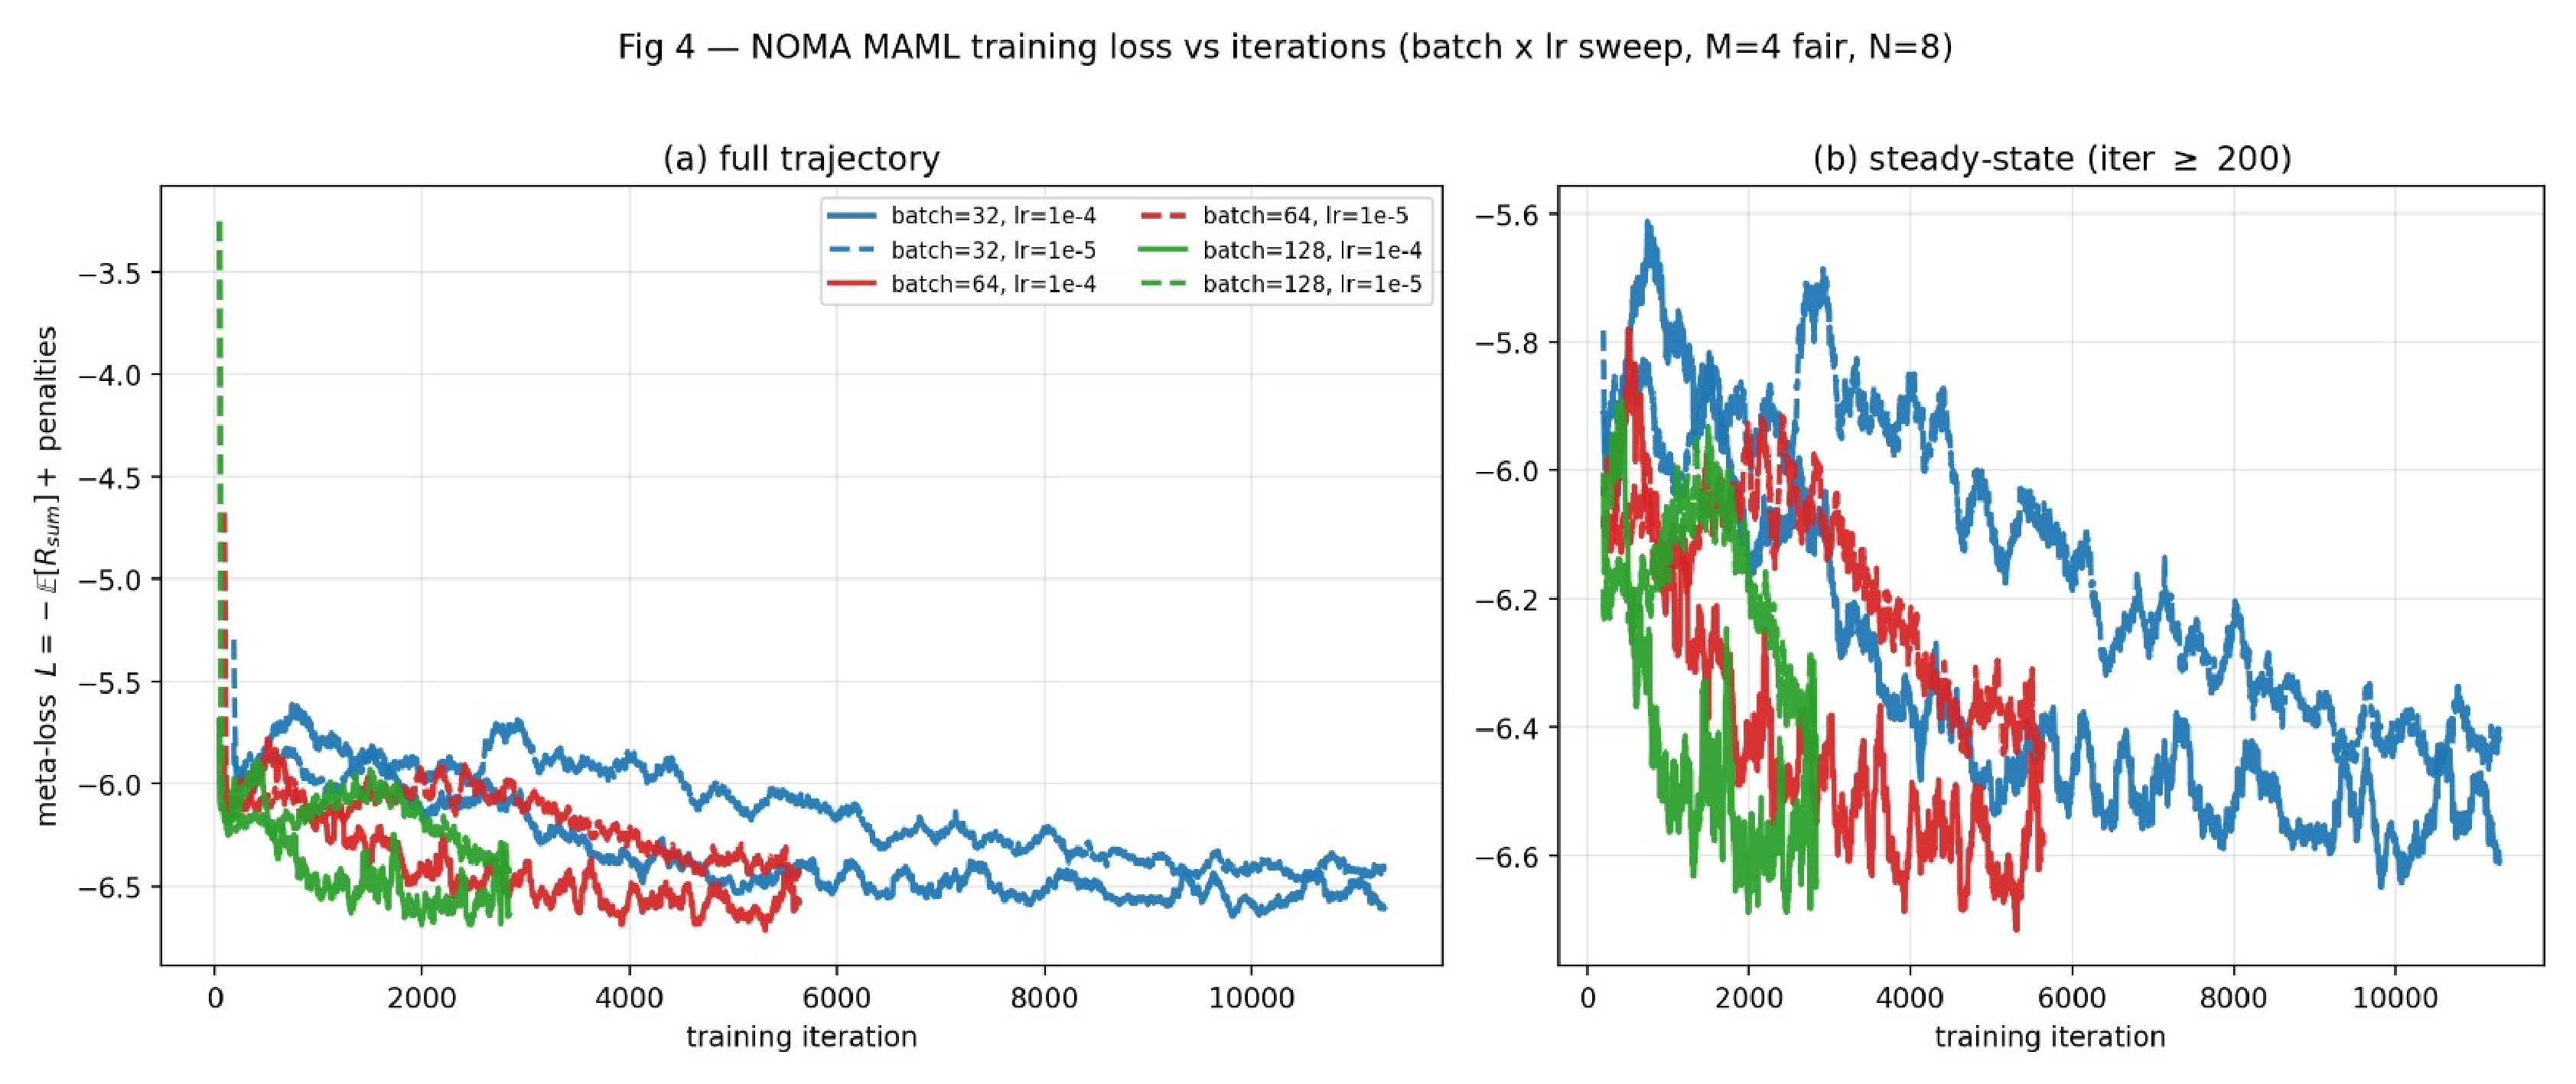
\includegraphics[width=\columnwidth]{fig_training}
  \caption{MAML meta-loss versus training iteration over a batch/learning-rate
  sweep ($M{=}4$, $N{=}8$). (a)~Full trajectory; (b)~steady state
  ($\text{iter}\!\ge\!200$).}
  \label{fig:training}
\end{figure}

Fig.~\ref{fig:cdf} plots the empirical CDF of the weighted sum-rate $\Rdl$ over
the test set for the ablation. Joint optimization of phase and power
(\textsf{fullOptimized}) stochastically dominates the partial designs, raising
the median from $\sim\!5.0$ to $\sim\!6.7$~bps/Hz; phase optimization accounts
for most of the rate gain, while the learned power split adds a further,
QoS-critical improvement. This is reflected in Fig.~\ref{fig:qos}: the joint
QoS-violation rate falls monotonically from $29.4\%$ (no optimization) to
$0.1\%$ (proposed), with both the communication ($q_c$) and sensing ($q_s$)
constraints satisfied almost surely.

\begin{figure}[t]
  \centering
  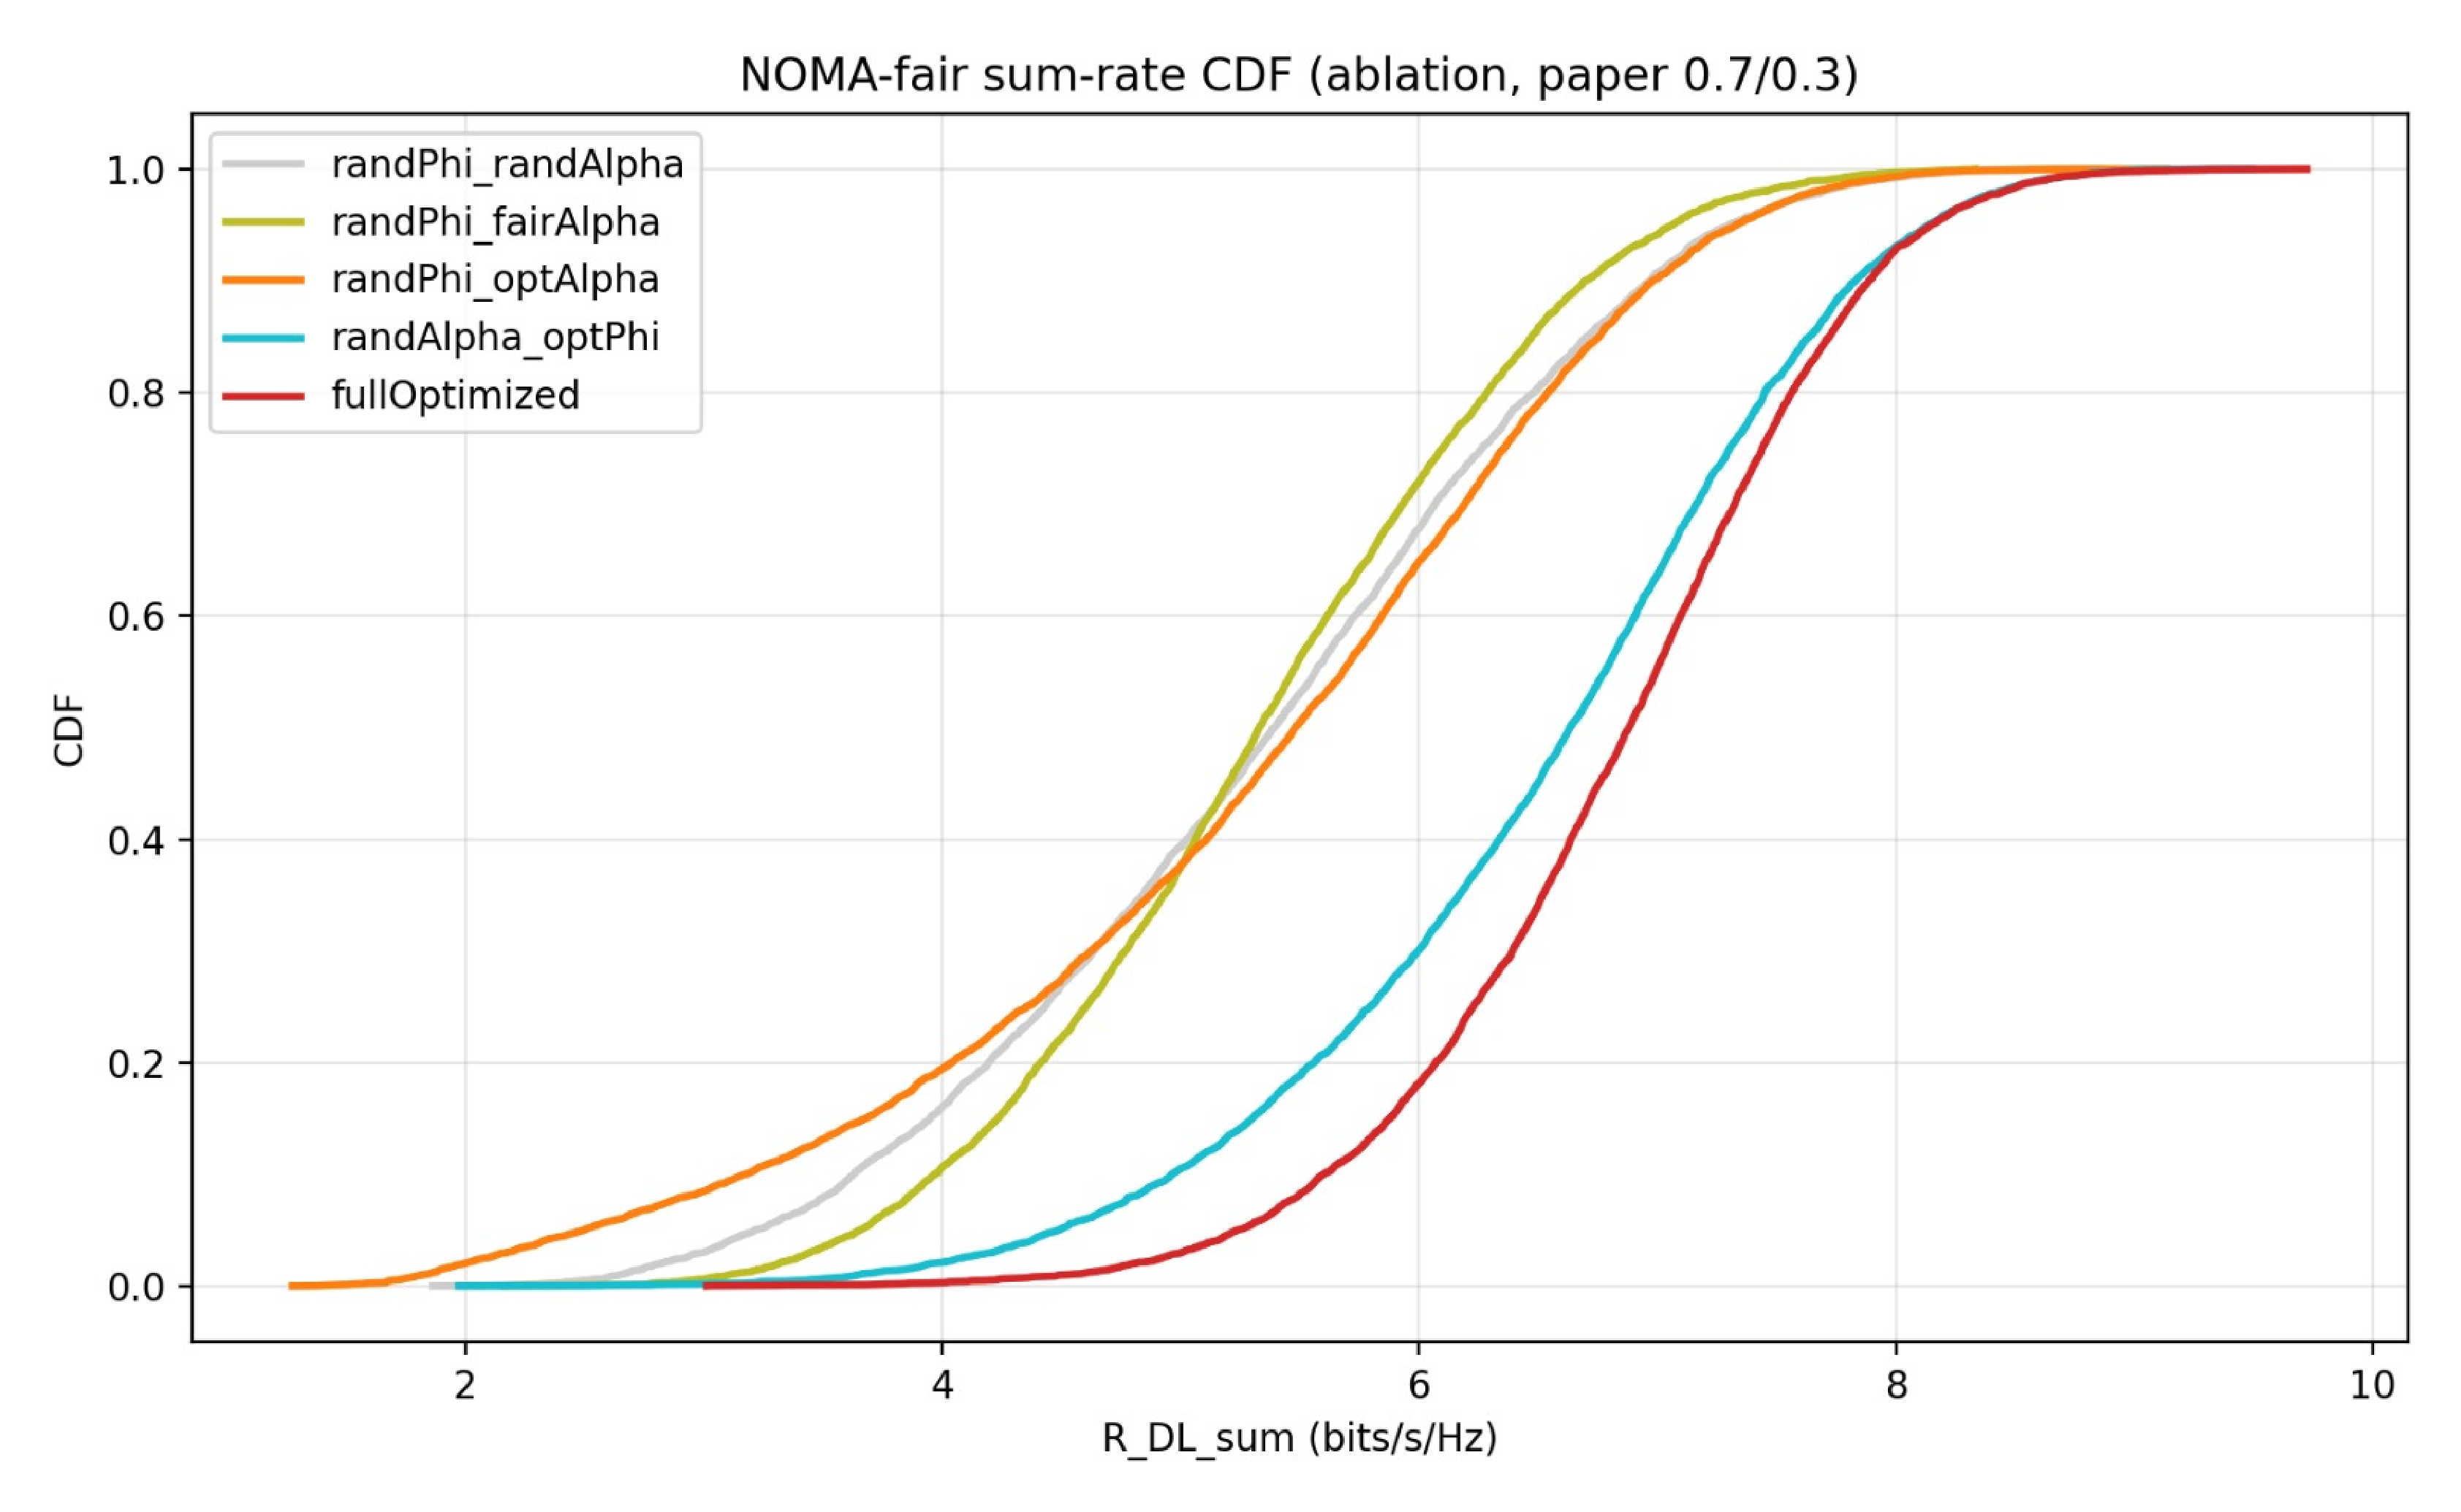
\includegraphics[width=\columnwidth]{fig_cdf}
  \caption{CDF of the weighted sum-rate $\Rdl$ over the test set for the five
  ablation configurations.}
  \label{fig:cdf}
\end{figure}

\begin{figure}[t]
  \centering
  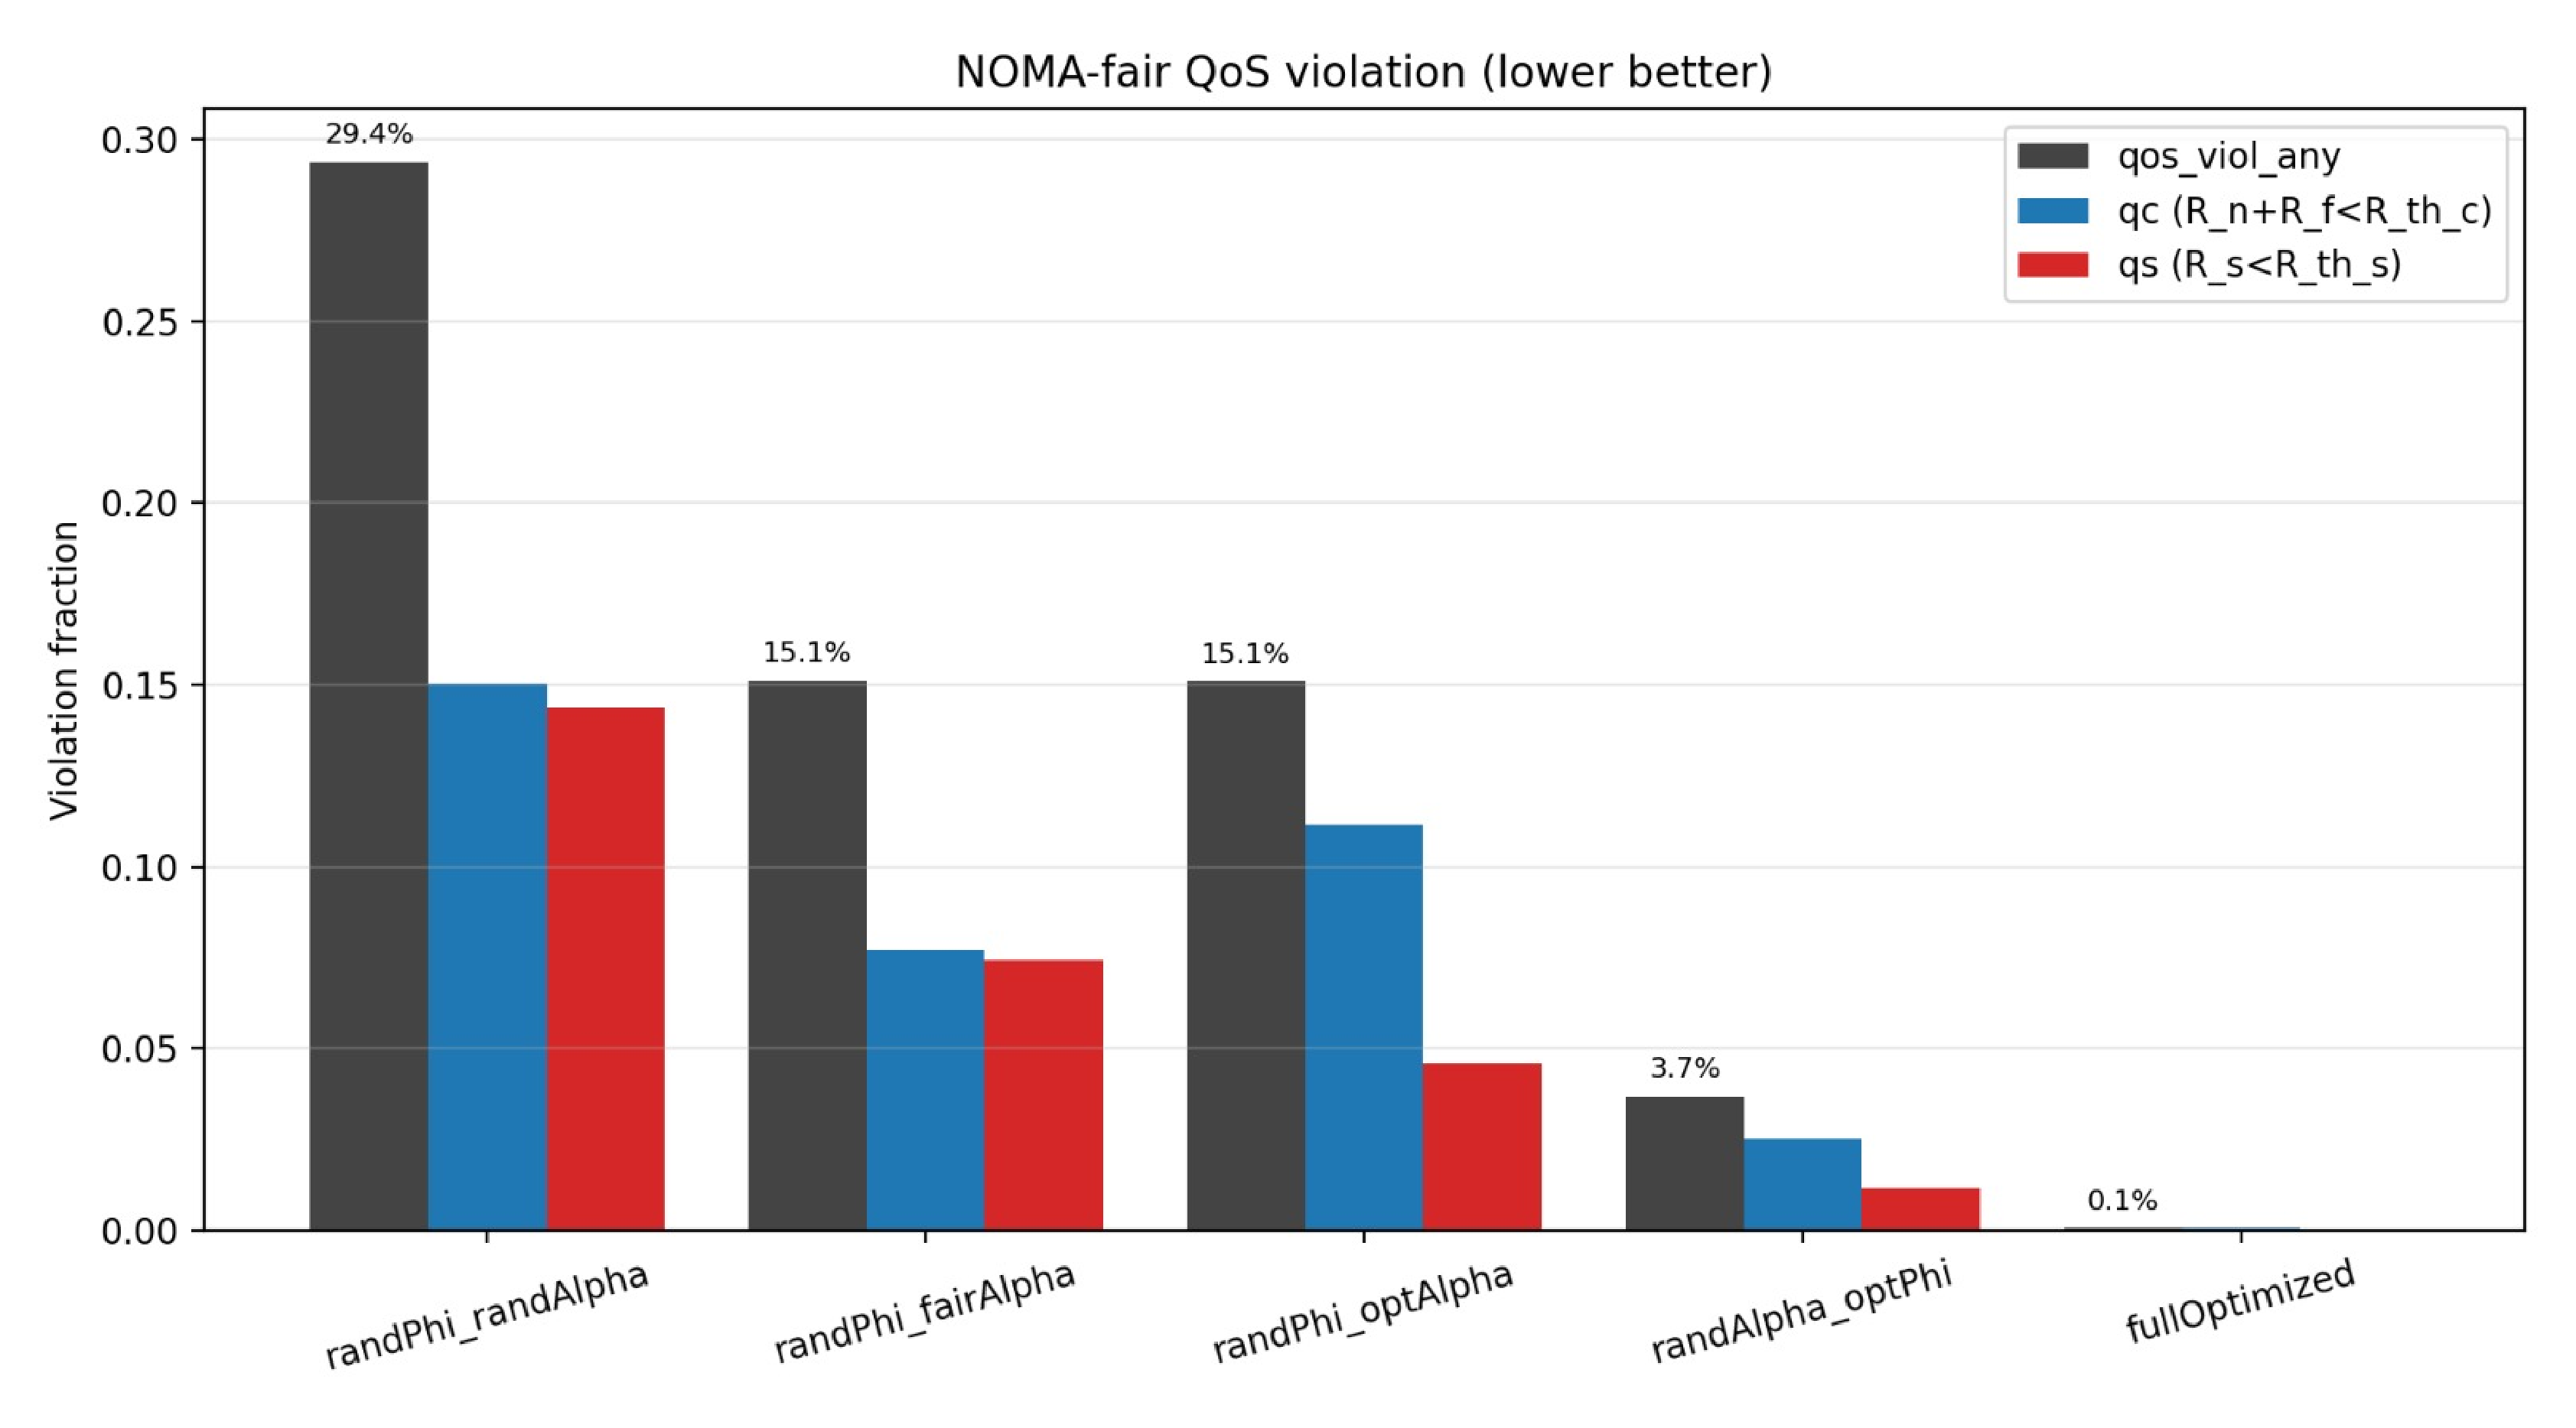
\includegraphics[width=\columnwidth]{fig_qos}
  \caption{QoS-violation fraction (lower is better). The joint violation rate
  drops from $29.4\%$ to $0.1\%$ along the ablation.}
  \label{fig:qos}
\end{figure}

% --- OPTIONAL extra ablation figures (uncomment to include) ------------------
% \begin{figure}[t]\centering
%   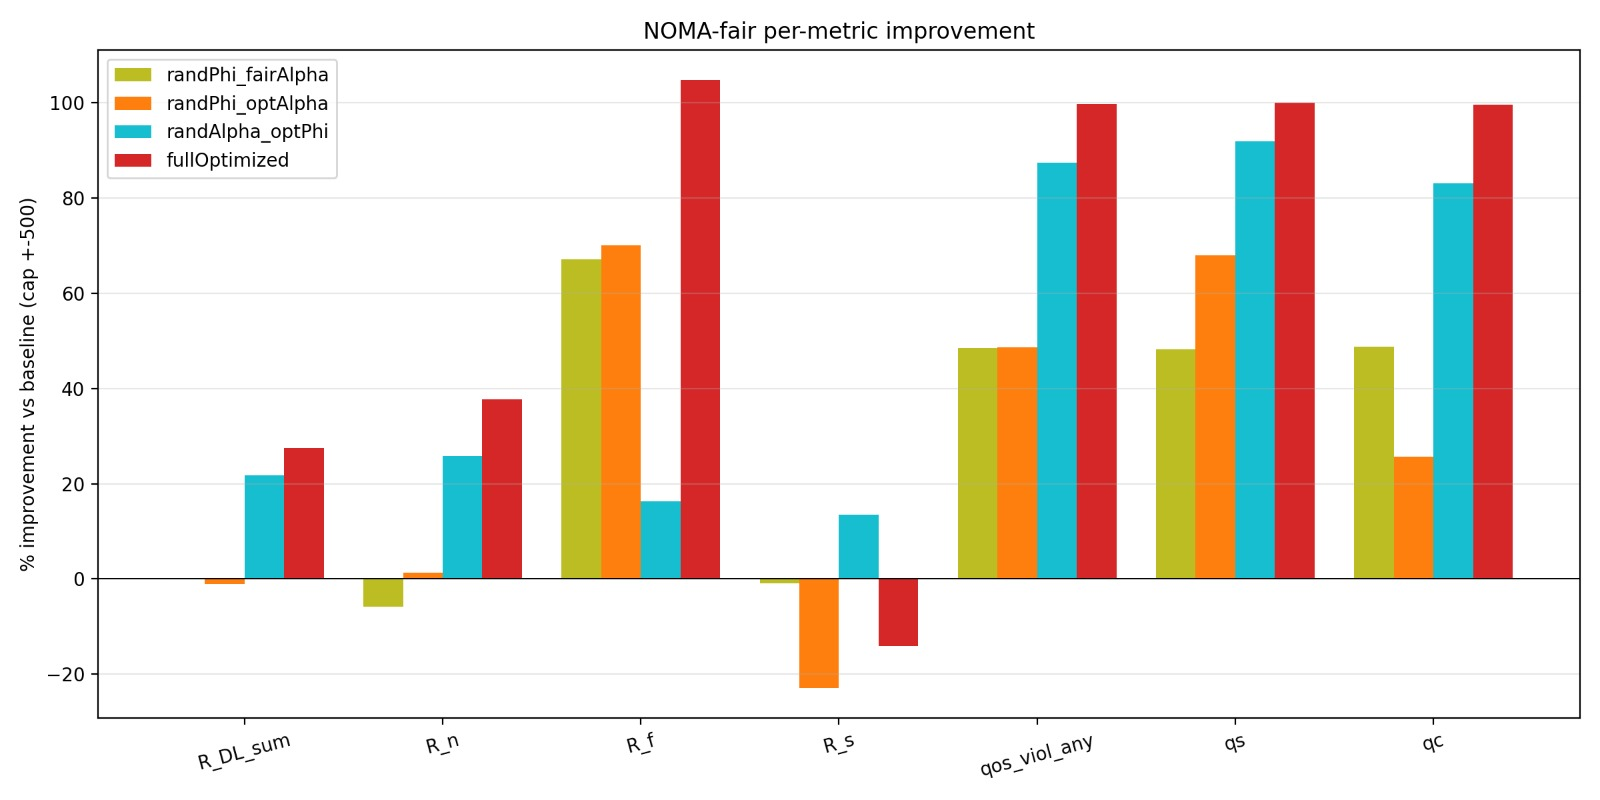
\includegraphics[width=\columnwidth]{fig_improvement.jpg}
%   \caption{Per-metric improvement over the unoptimized baseline.}\label{fig:improvement}\end{figure}
% \begin{figure}[t]\centering
%   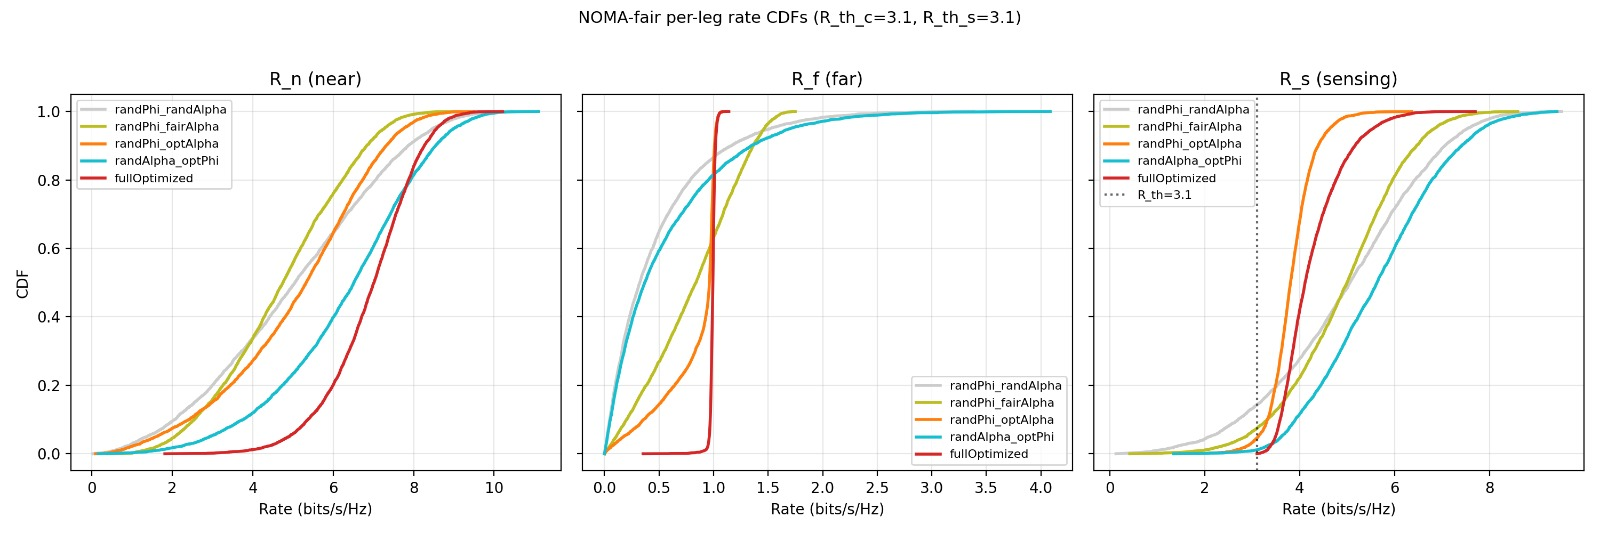
\includegraphics[width=\columnwidth]{fig_perleg.jpg}
%   \caption{Per-leg rate CDFs ($R_n$, $R_f$, $R_s$).}\label{fig:perleg}\end{figure}


Fig.~\ref{fig:rateN} reports $\Rsum$ versus the RIS size
$N\in\{8,16,32,64\}$ at $P=15$~dBm. The rate grows monotonically with $N$ for
both access schemes—from $6.9$ to $11.4$~bps/Hz for NOMA and from $4.1$ to
$7.3$~bps/Hz for OMA—and NOMA retains an $\sim\!65\%$ advantage throughout
showing that the passive aperture and the access scheme contribute complementary
gains.

\begin{figure}[t]
  \centering
  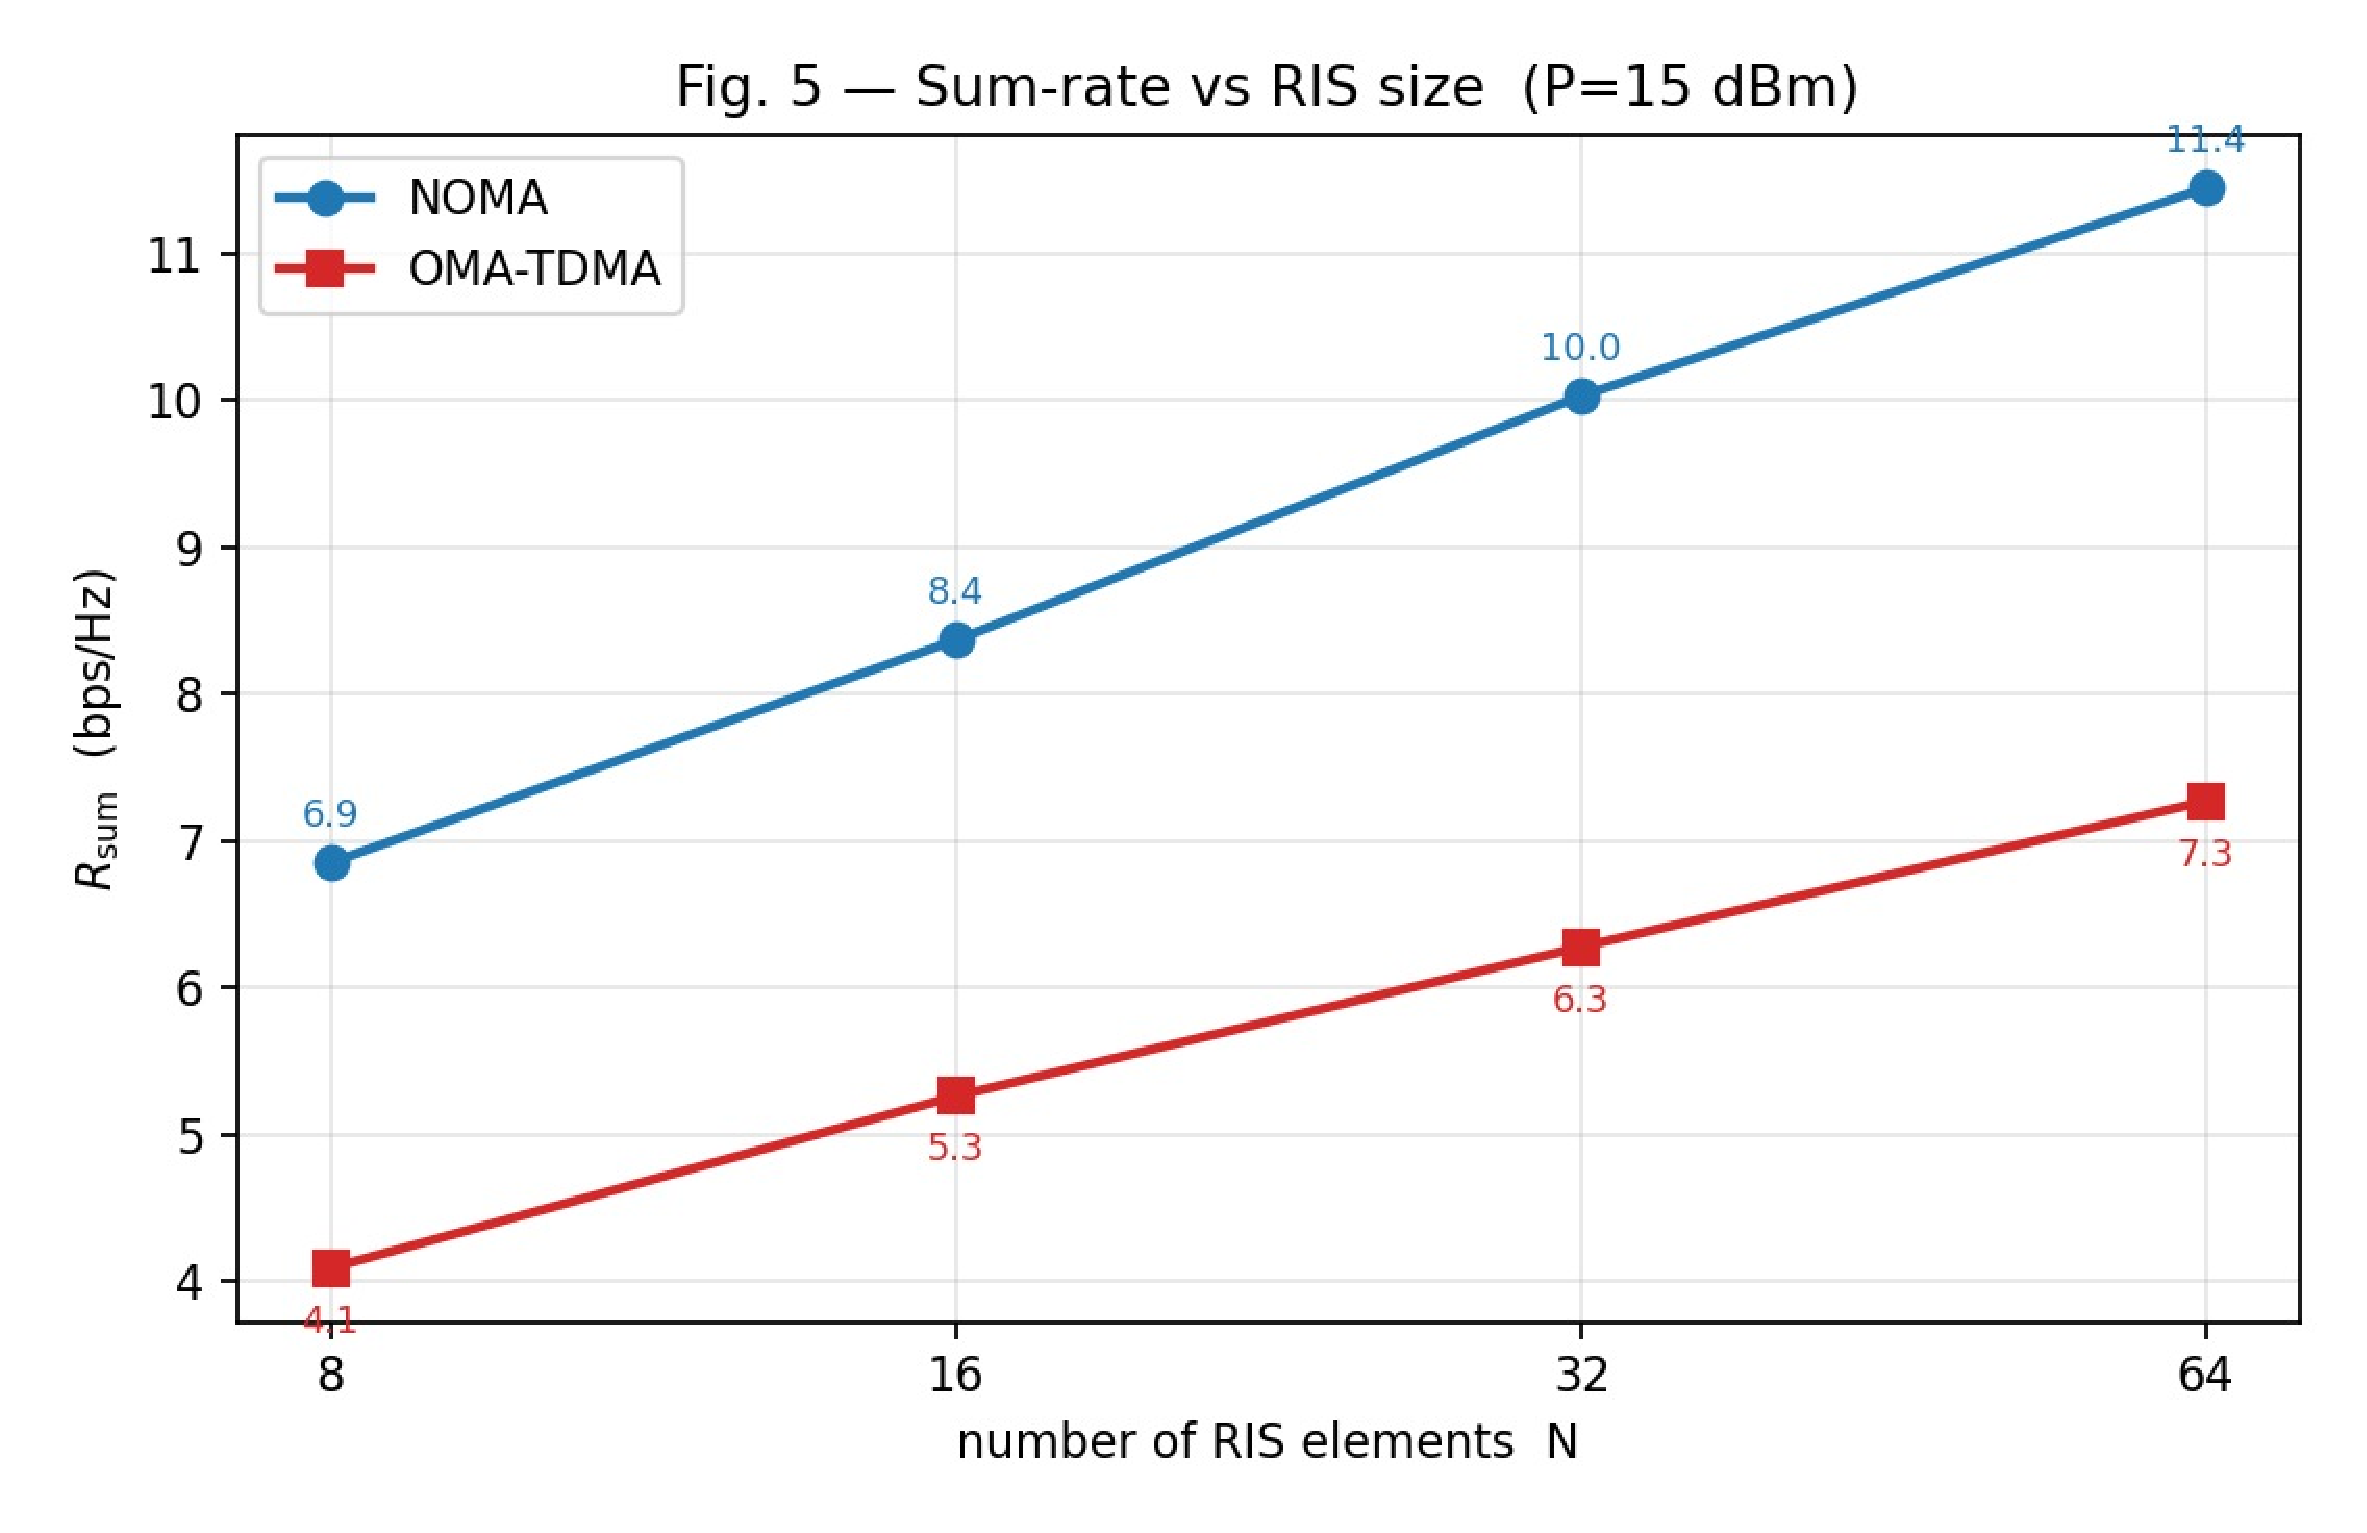
\includegraphics[width=\columnwidth]{fig_rate_N}
  \caption{Weighted sum-rate versus RIS size $N$ at $P=15$~dBm. NOMA dominates
  OMA at every aperture; both scale with $N$.}
  \label{fig:rateN}
\end{figure}
% REVIEWER ACTION PENDING DATA RERUN:
% Replace/add the requested six-policy NOMA comparison using:
% (1) proposed RIS+ML, (2) equal power+random RIS, (3) random power+random RIS,
% (4) equal power+fixed RIS, (5) random power+fixed RIS, (6) NOMA no-RIS.
% Do not fabricate these curves; generate them with the extended evaluator.


For the OMA references, the resource variable is a time-allocation vector
$\bm t=[t_n,t_f,t_T]$ rather than a NOMA power split. In the OMA--RIS branch,
the same shared RIS phase is adapted in the inner loop, the network predicts
$\bm t$ through a softmax layer, and the near/far slots use per-user MRT; the
sensing slot uses the dominant sensing direction. In the OMA no-RIS branch,
there is no phase variable, so the network predicts only the time fractions
from the direct-link features while retaining per-user MRT and the sensing
beam. Thus the OMA curves do not reuse the NOMA power-allocation policy.

Finally, Fig.~\ref{fig:rateP} sweeps the transmit power. Panel~(a) establishes
the ordering NOMA-RIS $>$ NOMA $>$ OMA-RIS $>$ OMA across the whole range:
NOMA's full-time superposition outperforms OMA's orthogonal slots, and the RIS
adds a consistent margin on top of each access scheme (e.g.\ a $\sim\!27\%$ RIS
gain for NOMA at $P=15$~dBm). Panel~(b) shows the corresponding QoS-violation
rate: NOMA-RIS reaches near-zero violation already at low power, whereas the
no-RIS and OMA schemes need substantially more power to become feasible,
quantifying the role of the RIS in jointly meeting the sensing and communication
QoS.

\begin{figure}[t]
  \centering
  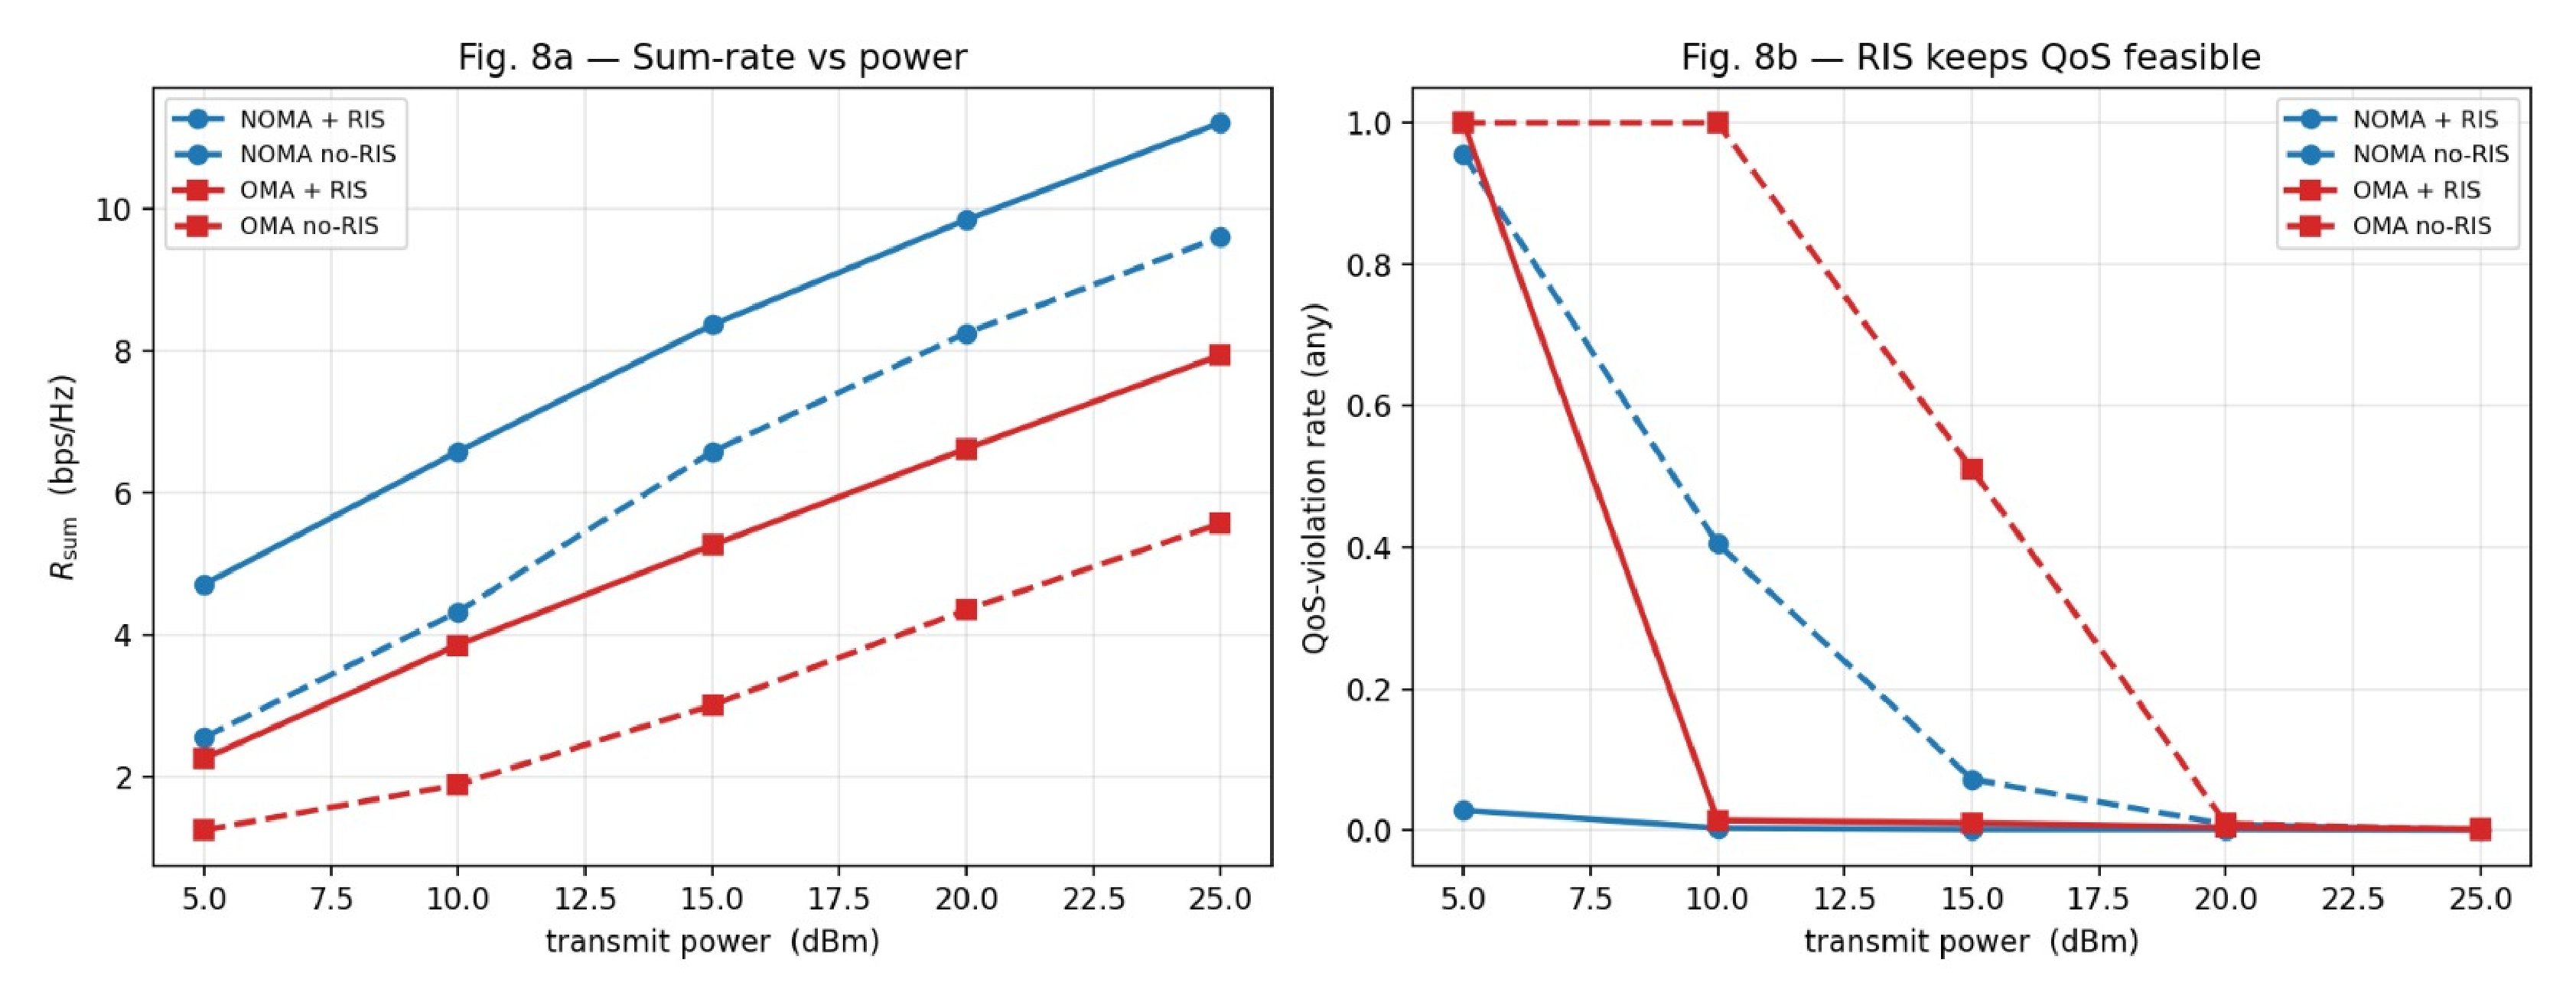
\includegraphics[width=\columnwidth]{fig_rate_P}
  \caption{(a)~Weighted sum-rate and (b)~joint QoS-violation rate versus
  transmit power for the four schemes.}
  \label{fig:rateP}
\end{figure}

Finally, two practical points follow. On \emph{runtime}, the online stage is a
single forward pass of $f_{\bm\theta}$ plus $K{=}5$ light inner steps---orders
of magnitude below per-instance AO---so the design fits the short coherence
times that motivate learning-based ISAC. On \emph{constraint granularity},
replacing the sum-rate floor \eqref{eq:qosc} with per-user penalties
($\lambda_n,\lambda_f{>}0$ in~\eqref{eq:sampleloss}) lets the operator dial the
near/far fairness trade-off, shifting the learned split toward the weaker user
at a modest cost in aggregate rate and with no change to the pipeline.


%==============================================================================
\section{Conclusion}
A MISO RIS-assisted NOMA-ISAC downlink was investigated with joint power and
phase design. The revised formulation combines an aggregate NOMA-cluster QoS
constraint with individual near/far-user floors and a separate sensing floor,
which preserves cluster efficiency while preventing a strong user from masking
a weak one. The implemented solver uses a compact softmax power network and
per-channel RIS-phase adaptation, followed by a first-order meta-update. The
paper now reports the actual channel distances, fading/path-loss parameters,
power/RIS settings, convergence limitations, and online prediction complexity.
The original result figures and their surrounding discussion are retained and the figure files are provided in EPS form for submission.

%==============================================================================
\begin{thebibliography}{1}
\bibitem{liu2022isac}
F.~Liu \emph{et al.}, ``Integrated sensing and communications: Toward
dual-functional wireless networks for 6G and beyond,''
\emph{IEEE J. Sel. Areas Commun.}, vol.~40, no.~6, pp.~1728--1767, Jun.~2022.

\bibitem{deng2025mmwave}
K.~Deng, X.~Wang, H.~Xu, Q.~Song, R.~Zhang, and Y.~Qian, ``Balancing
communication and sensing hybrid beamforming with rank-1 optimization for
mmWave ISAC systems,'' \emph{IEEE Wireless Commun. Lett.}, vol.~14, no.~9,
pp.~2738--2742, Sep.~2025.

\bibitem{wu2020ris}
Q.~Wu and R.~Zhang, ``Towards smart and reconfigurable environment: Intelligent
reflecting surface aided wireless network,'' \emph{IEEE Commun. Mag.}, vol.~58,
no.~1, pp.~106--112, Jan.~2020.

\bibitem{wang2025hybrid}
L.~Wang, L.~F. Abanto-Leon, and A.~Asadi, ``Joint hybrid beamforming and RIS
phase shift design for RIS-enabled mmWave ISAC system,'' \emph{IEEE Trans. Veh.
Technol.}, vol.~74, no.~6, pp.~9149--9164, Jun.~2025.

\bibitem{lyu2024crb}
W.~Lyu \emph{et al.}, ``CRB minimization for RIS-aided mmWave integrated sensing
and communications,'' \emph{IEEE Internet Things J.}, vol.~11, no.~10,
pp.~18381--18393, May~2024.

\bibitem{ke2025rsma}
H.~Ke, J.~Xu, W.~Xu, C.~Ding, and D.~W.~K. Ng, ``Rate splitting and beamforming
design for RIS-assisted RSMA-enhanced ISAC networks,'' \emph{IEEE Wireless
Commun. Lett.}, vol.~14, no.~6, pp.~1738--1742, Jun.~2025.

\bibitem{zou2023ml}
Y.~Zou, Y.~Liu, X.~Mu, X.~Zhang, Y.~Liu, and C.~Yuen, ``Machine learning in
RIS-assisted NOMA IoT networks,'' \emph{IEEE Internet Things J.}, vol.~10,
no.~22, pp.~19427--19440, Nov.~2023.

\bibitem{wei2026ris}
T.~Wei \emph{et al.}, ``Machine learning-driven joint RIS partitioning,
beamforming, and phase shifts design for mmWave ISAC systems,'' \emph{IEEE
Wireless Commun. Lett.}, vol.~15, 2026.

\bibitem{maml}
C.~Finn, P.~Abbeel, and S.~Levine, ``Model-agnostic meta-learning for fast
adaptation of deep networks,'' in \emph{Proc. ICML}, 2017, pp.~1126--1135.

\bibitem{fallah2020maml}
A.~Fallah, A.~Mokhtari, and A.~Ozdaglar, ``On the convergence theory of
gradient-based model-agnostic meta-learning algorithms,'' in \emph{Proc.
AISTATS}, 2020, pp.~1082--1092.

\bibitem{ji2022maml}
K.~Ji, J.~Yang, and Y.~Liang, ``Theoretical convergence of multi-step
model-agnostic meta-learning,'' \emph{J. Mach. Learn. Res.}, vol.~23, pp.~1--41,
2022.

\bibitem{sun2024noma}
Y.~Sun \emph{et al.}, ``On the study of NOMA-assisted integrated sensing and
communication networks,'' \emph{IEEE Trans. Commun.}, vol.~72, no.~11,
pp.~7278--7293, Nov.~2024.

\bibitem{basar2019ris}
E.~Basar, M.~Di Renzo, J.~de Rosny, M.~Debbah, M.-S. Alouini, and R.~Zhang,
"Wireless communications through reconfigurable intelligent surfaces,"
\emph{IEEE Access}, vol.~7, pp.~116753--116773, 2019.

\bibitem{ding2017noma}
Z.~Ding, X.~Lei, G.~K. Karagiannidis, R.~Schober, J.~Yuan, and V.~K. Bhargava,
"A survey on non-orthogonal multiple access for 5G networks: Research
challenges and future trends," \emph{IEEE J. Sel. Areas Commun.}, vol.~35,
no.~10, pp.~2181--2195, Oct.~2017.

\bibitem{hospedales2022meta}
T.~M. Hospedales, A.~Antoniou, P.~Micaelli, and A.~J. Storkey,
"Meta-learning in neural networks: A survey," \emph{IEEE Trans. Pattern Anal.
Mach. Intell.}, vol.~44, no.~9, pp.~5149--5169, Sep.~2022.

\end{thebibliography}

\end{document}
